%\immediate\write18{specifications/figs/make_axial_figs.py}

While some of the previously-described radial features are uniform along the
entire height of the model, many have several different axial zones. For
instance, the models of the baffle, core barrel, neutron shield panels, and
reactor pressure vessel do not change axially, in contrast to the pincells
that make up the fuel assemblies. As presented in the following sections, the
axial zones are treated at the pincell level to facilitate easier modelling,
since the boundaries for the axial zones for each pincell type are not all at
the same planes. With this type of definition, the final aggregate geometry
inside the core barrel need only consist of the fuel assemblies, which are made
up of only the inter-assembly gridstraps and the pincells that are defined for
the entire axial extent.

%%%%%%%%%%%%%%%%%%%%%%%%%%%%%%%%%%%%%%%%%%%%%%%%%%%%%%%%%%%%%%%%%%%%%%%%%%%%%%%%
\subsubsection{Fuel Rods}

Figure \ref{fig_fuel_axials} shows all different axial sections used in the fuel
rod pincell occupying each fuel position in the assemblies.  In most
places the pincells described in Section \ref{sec:pintypes} are used, however
where indicated the pincell is filled either entirely with water, or with solid
pins of either stainless steel or Zircaloy.  These solid pins use the outer-most
radius of the regular fuel rod pincell.

\begin{figure}[htbp]
    \centering
    \begin{tikzpicture}[scale=1,x=1in,y=1in]
      \node[inner sep=0pt,
        text width=3 in,
        minimum size=0.2 in,
        draw=black,
        align=center,
        shift={(0,0.0)},
        hyperlink node=mat_water] (n0) {Water};
      \draw[->] (1.7,-0.1) node[right,anchor=west] {0.00000 ~~~~~~~ Lowest Extent} -- (1.5,-0.1);
      \node[anchor=east] (s0) at (n0.west) {};
      \node[inner sep=0pt,
        text width=3 in,
        minimum size=0.2 in,
        draw=black,
        align=center,
        shift={(0,0.2)},
        hyperlink node=mat_ss_spn] (n1) {Nozzle / Support Plate Stainless Steel};
      \draw[->] (1.7,0.1) node[right,anchor=west] {20.0000 ~~~~~~~ Bottom of Support Plate} -- (1.5,0.1);
      \node[anchor=east] (s1) at (n1.west) {\ref{num:missing}};
      \node[inner sep=0pt,
        text width=3 in,
        minimum size=0.2 in,
        draw=black,
        align=center,
        shift={(0,0.4)},
        hyperlink node=mat_zirc] (n2) {Zircaloy Pin};
      \draw[->] (1.7,0.3) node[right,anchor=west] {35.0000 ~~~~~~~ Bottom of Fuel Rod} -- (1.5,0.3);
      \node[anchor=east] (s2) at (n2.west) {\ref{num:catawba}};
      \node[inner sep=0pt,
        text width=3 in,
        minimum size=0.2 in,
        draw=black,
        align=center,
        shift={(0,0.6)},
        hyperlink node=fig_fuel_pin] (n3) {Fuel Rod Pincell};
      \draw[->] (1.7,0.5) node[right,anchor=west] {36.7480 ~~~~~~~ Bottom of Active Fuel} -- (1.5,0.5);
      \node[anchor=east] (s3) at (n3.west) {\ref{num:fuelheight}};
      \node[inner sep=0pt,
        text width=3 in,
        minimum size=0.2 in,
        draw=black,
        align=center,
        shift={(0,0.8)},
        hyperlink node=grid_spec] (n4) {Fuel Rod Pincell w/ Grid};
      \draw[->] (1.7,0.7) node[right,anchor=west] {37.1621 ~~~~~~~ Grid 1 Bottom} -- (1.5,0.7);
      \node[anchor=east] (s4) at (n4.west) {\ref{num:grid_spacer}};
      \node[inner sep=0pt,
        text width=3 in,
        minimum size=0.2 in,
        draw=black,
        align=center,
        shift={(0,1.0)},
        hyperlink node=fig_fuel_pin] (n5) {Fuel Rod Pincell};
      \draw[->] (1.7,0.9) node[right,anchor=west] {40.5200 ~~~~~~~ Grid 1 Top} -- (1.5,0.9);
      \node[anchor=east] (s5) at (n5.west) {\ref{num:fuelheight}};
      \node[inner sep=0pt,
        text width=3 in,
        minimum size=0.2 in,
        draw=black,
        align=center,
        shift={(0,1.2)},
        hyperlink node=grid_spec] (n6) {Fuel Rod Pincell w/ Grid};
      \draw[->] (1.7,1.1) node[right,anchor=west] {98.0250 ~~~~~~~ Grid 2 Bottom} -- (1.5,1.1);
      \node[anchor=east] (s6) at (n6.west) {\ref{num:grid_spacer}};
      \node[inner sep=0pt,
        text width=3 in,
        minimum size=0.2 in,
        draw=black,
        align=center,
        shift={(0,1.4)},
        hyperlink node=fig_fuel_pin] (n7) {Fuel Rod Pincell};
      \draw[->] (1.7,1.3) node[right,anchor=west] {103.740 ~~~~~~~ Grid 2 Top} -- (1.5,1.3);
      \node[anchor=east] (s7) at (n7.west) {\ref{num:fuelheight}};
      \node[inner sep=0pt,
        text width=3 in,
        minimum size=0.2 in,
        draw=black,
        align=center,
        shift={(0,1.6)},
        hyperlink node=grid_spec] (n8) {Fuel Rod Pincell w/ Grid};
      \draw[->] (1.7,1.5) node[right,anchor=west] {150.222 ~~~~~~~ Grid 3 Bottom} -- (1.5,1.5);
      \node[anchor=east] (s8) at (n8.west) {\ref{num:grid_spacer}};
      \node[inner sep=0pt,
        text width=3 in,
        minimum size=0.2 in,
        draw=black,
        align=center,
        shift={(0,1.8)},
        hyperlink node=fig_fuel_pin] (n9) {Fuel Rod Pincell};
      \draw[->] (1.7,1.7) node[right,anchor=west] {155.937 ~~~~~~~ Grid 3 Top} -- (1.5,1.7);
      \node[anchor=east] (s9) at (n9.west) {\ref{num:fuelheight}};
      \node[inner sep=0pt,
        text width=3 in,
        minimum size=0.2 in,
        draw=black,
        align=center,
        shift={(0,2.0)},
        hyperlink node=grid_spec] (n10) {Fuel Rod Pincell w/ Grid};
      \draw[->] (1.7,1.9) node[right,anchor=west] {202.419 ~~~~~~~ Grid 4 Bottom} -- (1.5,1.9);
      \node[anchor=east] (s10) at (n10.west) {\ref{num:grid_spacer}};
      \node[inner sep=0pt,
        text width=3 in,
        minimum size=0.2 in,
        draw=black,
        align=center,
        shift={(0,2.2)},
        hyperlink node=fig_fuel_pin] (n11) {Fuel Rod Pincell};
      \draw[->] (1.7,2.1) node[right,anchor=west] {208.134 ~~~~~~~ Grid 4 Top} -- (1.5,2.1);
      \node[anchor=east] (s11) at (n11.west) {\ref{num:fuelheight}};
      \node[inner sep=0pt,
        text width=3 in,
        minimum size=0.2 in,
        draw=black,
        align=center,
        shift={(0,2.4)},
        hyperlink node=grid_spec] (n12) {Fuel Rod Pincell w/ Grid};
      \draw[->] (1.7,2.3) node[right,anchor=west] {254.616 ~~~~~~~ Grid 5 Bottom} -- (1.5,2.3);
      \node[anchor=east] (s12) at (n12.west) {\ref{num:grid_spacer}};
      \node[inner sep=0pt,
        text width=3 in,
        minimum size=0.2 in,
        draw=black,
        align=center,
        shift={(0,2.6)},
        hyperlink node=fig_fuel_pin] (n13) {Fuel Rod Pincell};
      \draw[->] (1.7,2.5) node[right,anchor=west] {260.331 ~~~~~~~ Grid 5 Top} -- (1.5,2.5);
      \node[anchor=east] (s13) at (n13.west) {\ref{num:fuelheight}};
      \node[inner sep=0pt,
        text width=3 in,
        minimum size=0.2 in,
        draw=black,
        align=center,
        shift={(0,2.8)},
        hyperlink node=grid_spec] (n14) {Fuel Rod Pincell w/ Grid};
      \draw[->] (1.7,2.7) node[right,anchor=west] {306.813 ~~~~~~~ Grid 6 Bottom} -- (1.5,2.7);
      \node[anchor=east] (s14) at (n14.west) {\ref{num:grid_spacer}};
      \node[inner sep=0pt,
        text width=3 in,
        minimum size=0.2 in,
        draw=black,
        align=center,
        shift={(0,3.0)},
        hyperlink node=fig_fuel_pin] (n15) {Fuel Rod Pincell};
      \draw[->] (1.7,2.9) node[right,anchor=west] {312.528 ~~~~~~~ Grid 6 Top} -- (1.5,2.9);
      \node[anchor=east] (s15) at (n15.west) {\ref{num:fuelheight}};
      \node[inner sep=0pt,
        text width=3 in,
        minimum size=0.2 in,
        draw=black,
        align=center,
        shift={(0,3.2)},
        hyperlink node=grid_spec] (n16) {Fuel Rod Pincell w/ Grid};
      \draw[->] (1.7,3.1) node[right,anchor=west] {359.010 ~~~~~~~ Grid 7 Bottom} -- (1.5,3.1);
      \node[anchor=east] (s16) at (n16.west) {\ref{num:grid_spacer}};
      \node[inner sep=0pt,
        text width=3 in,
        minimum size=0.2 in,
        draw=black,
        align=center,
        shift={(0,3.4)},
        hyperlink node=fig_fuel_pin] (n17) {Fuel Rod Pincell};
      \draw[->] (1.7,3.3) node[right,anchor=west] {364.725 ~~~~~~~ Grid 7 Top} -- (1.5,3.3);
      \node[anchor=east] (s17) at (n17.west) {\ref{num:fuelheight}};
      \node[inner sep=0pt,
        text width=3 in,
        minimum size=0.2 in,
        draw=black,
        align=center,
        shift={(0,3.6)},
        hyperlink node=fig_fuel_pin] (n18) {Fuel Rod Plenum Pincell};
      \draw[->] (1.7,3.5) node[right,anchor=west] {402.508 ~~~~~~~ Top of Active Fuel} -- (1.5,3.5);
      \node[anchor=east] (s18) at (n18.west) {\ref{num:catawba}};
      \node[inner sep=0pt,
        text width=3 in,
        minimum size=0.2 in,
        draw=black,
        align=center,
        shift={(0,3.8)},
        hyperlink node=grid_spec] (n19) {Fuel Rod Plenum Pincell w/ Grid};
      \draw[->] (1.7,3.7) node[right,anchor=west] {411.806 ~~~~~~~ Grid 8 Bottom} -- (1.5,3.7);
      \node[anchor=east] (s19) at (n19.west) {\ref{num:grid_spacer}};
      \node[inner sep=0pt,
        text width=3 in,
        minimum size=0.2 in,
        draw=black,
        align=center,
        shift={(0,4.0)},
        hyperlink node=fig_fuel_pin] (n20) {Fuel Rod Plenum Pincell};
      \draw[->] (1.7,3.9) node[right,anchor=west] {415.164 ~~~~~~~ Grid 8 Top} -- (1.5,3.9);
      \node[anchor=east] (s20) at (n20.west) {\ref{num:catawba}};
      \node[inner sep=0pt,
        text width=3 in,
        minimum size=0.2 in,
        draw=black,
        align=center,
        shift={(0,4.2)},
        hyperlink node=mat_zirc] (n21) {Zircaloy Pin};
      \draw[->] (1.7,4.1) node[right,anchor=west] {417.164 ~~~~~~~ Top of Fuel Rod Plenum} -- (1.5,4.1);
      \node[anchor=east] (s21) at (n21.west) {\ref{num:catawba}};
      \node[inner sep=0pt,
        text width=3 in,
        minimum size=0.2 in,
        draw=black,
        align=center,
        shift={(0,4.4)},
        hyperlink node=mat_water] (n22) {Water};
      \draw[->] (1.7,4.3) node[right,anchor=west] {419.704 ~~~~~~~ Top of Fuel Rod} -- (1.5,4.3);
      \node[anchor=east] (s22) at (n22.west) {\ref{num:catawba}};
      \node[inner sep=0pt,
        text width=3 in,
        minimum size=0.2 in,
        draw=black,
        align=center,
        shift={(0,4.6)},
        hyperlink node=mat_ss_spn] (n23) {Nozzle / Support Plate Stainless Steel};
      \draw[->] (1.7,4.5) node[right,anchor=west] {423.049 ~~~~~~~ Bottom of Upper Nozzle} -- (1.5,4.5);
      \node[anchor=east] (s23) at (n23.west) {\ref{num:watts_bar}};
      \node[inner sep=0pt,
        text width=3 in,
        minimum size=0.2 in,
        draw=black,
        align=center,
        shift={(0,4.8)},
        hyperlink node=mat_water] (n24) {Water};
      \draw[->] (1.7,4.7) node[right,anchor=west] {431.876 ~~~~~~~ Top of Upper Nozzle} -- (1.5,4.7);
      \node[anchor=east] (s24) at (n24.west) {\ref{num:watts_bar}};
      \path let \p1 = (n24.west) in node[anchor=west] (source) at (\x1,5.1) {\underline{Source Reference}};
      \draw[->] (source.west) -| (s24.north);
      \draw[->] (1.7,4.9) node[right,anchor=west] {460.000 ~~~~~~~ Highest Extent} -- (1.5,4.9);
      \draw (1.5,5.1) node[right,anchor=west] {\underline{Elevation (cm)} ~ \underline{Description}};

    \end{tikzpicture}


    \caption[Fuel rod pincell axial specification]{Fuel rod pincell axial specification.\label{fig_fuel_axials}}
\end{figure} % label: fig_fuel_axials

%%%%%%%%%%%%%%%%%%%%%%%%%%%%%%%%%%%%%%%%%%%%%%%%%%%%%%%%%%%%%%%%%%%%%%%%%%%%%%%%
\subsubsection{Guide Tubes}

Figure \ref{fig_gtu_axials} shows the empty guide tube axial differentiation,
referring to the pincells described in Section \ref{sec:pintypes}.  As with
the fuel rods, the pincell is replaced by water below the fuel region.

\begin{figure}[htbp]
    \centering
    \begin{tikzpicture}[scale=1,x=1in,y=1in]
      \node[inner sep=0pt,
        text width=3 in,
        minimum size=0.227272727273 in,
        draw=black,
        align=center,
        shift={(0,0.0)},
        hyperlink node=mat_water] (n0) {Water};
      \draw[->] (1.7,-0.113636363636) node[right,anchor=west] {0.00000 ~~~~~~~ Lowest Extent} -- (1.5,-0.113636363636);
      \node[anchor=east] (s0) at (n0.west) {};
      \node[inner sep=0pt,
        text width=3 in,
        minimum size=0.227272727273 in,
        draw=black,
        align=center,
        shift={(0,0.227272727273)},
        hyperlink node=mat_water_spn] (n1) {Nozzle / Support Plate Borated Water};
      \draw[->] (1.7,0.113636363636) node[right,anchor=west] {20.0000 ~~~~~~~ Bottom of Support Plate} -- (1.5,0.113636363636);
      \node[anchor=east] (s1) at (n1.west) {\ref{num:missing}};
      \node[inner sep=0pt,
        text width=3 in,
        minimum size=0.227272727273 in,
        draw=black,
        align=center,
        shift={(0,0.454545454545)},
        hyperlink node=fig_guidetube_da_pin] (n2) {Dashpot Guide Tube};
      \draw[->] (1.7,0.340909090909) node[right,anchor=west] {35.0000 ~~~~~~~ Bottom of Fuel Rod} -- (1.5,0.340909090909);
      \node[anchor=east] (s2) at (n2.west) {\ref{num:gtu_axials}};
      \node[inner sep=0pt,
        text width=3 in,
        minimum size=0.227272727273 in,
        draw=black,
        align=center,
        shift={(0,0.681818181818)},
        hyperlink node=fig_guidetube_da_pin] (n3) {Dashpot Guide Tube w/ Grid};
      \draw[->] (1.7,0.568181818182) node[right,anchor=west] {37.1621 ~~~~~~~ Grid 1 Bottom} -- (1.5,0.568181818182);
      \node[anchor=east] (s3) at (n3.west) {\ref{num:gtu_axials}};
      \node[inner sep=0pt,
        text width=3 in,
        minimum size=0.227272727273 in,
        draw=black,
        align=center,
        shift={(0,0.909090909091)},
        hyperlink node=grid_spec] (n4) {Guide Tube Pincell w/ Grid};
      \draw[->] (1.7,0.795454545455) node[right,anchor=west] {39.9580 ~~~~~~~ Control Rod Step 0} -- (1.5,0.795454545455);
      \node[anchor=east] (s4) at (n4.west) {\ref{num:grid_spacer}};
      \node[inner sep=0pt,
        text width=3 in,
        minimum size=0.227272727273 in,
        draw=black,
        align=center,
        shift={(0,1.13636363636)},
        hyperlink node=fig_guidetube_pin] (n5) {Guide Tube Pincell};
      \draw[->] (1.7,1.02272727273) node[right,anchor=west] {40.5200 ~~~~~~~ Grid 1 Top} -- (1.5,1.02272727273);
      \node[anchor=east] (s5) at (n5.west) {\ref{num:gtu_axials}};
      \node[inner sep=0pt,
        text width=3 in,
        minimum size=0.227272727273 in,
        draw=black,
        align=center,
        shift={(0,1.36363636364)},
        hyperlink node=grid_spec] (n6) {Guide Tube Pincell w/ Grid};
      \draw[->] (1.7,1.25) node[right,anchor=west] {98.0250 ~~~~~~~ Grid 2 Bottom} -- (1.5,1.25);
      \node[anchor=east] (s6) at (n6.west) {\ref{num:grid_spacer}};
      \node[inner sep=0pt,
        text width=3 in,
        minimum size=0.227272727273 in,
        draw=black,
        align=center,
        shift={(0,1.59090909091)},
        hyperlink node=fig_guidetube_pin] (n7) {Guide Tube Pincell};
      \draw[->] (1.7,1.47727272727) node[right,anchor=west] {103.740 ~~~~~~~ Grid 2 Top} -- (1.5,1.47727272727);
      \node[anchor=east] (s7) at (n7.west) {\ref{num:gtu_axials}};
      \node[inner sep=0pt,
        text width=3 in,
        minimum size=0.227272727273 in,
        draw=black,
        align=center,
        shift={(0,1.81818181818)},
        hyperlink node=grid_spec] (n8) {Guide Tube Pincell w/ Grid};
      \draw[->] (1.7,1.70454545455) node[right,anchor=west] {150.222 ~~~~~~~ Grid 3 Bottom} -- (1.5,1.70454545455);
      \node[anchor=east] (s8) at (n8.west) {\ref{num:grid_spacer}};
      \node[inner sep=0pt,
        text width=3 in,
        minimum size=0.227272727273 in,
        draw=black,
        align=center,
        shift={(0,2.04545454545)},
        hyperlink node=fig_guidetube_pin] (n9) {Guide Tube Pincell};
      \draw[->] (1.7,1.93181818182) node[right,anchor=west] {155.937 ~~~~~~~ Grid 3 Top} -- (1.5,1.93181818182);
      \node[anchor=east] (s9) at (n9.west) {\ref{num:gtu_axials}};
      \node[inner sep=0pt,
        text width=3 in,
        minimum size=0.227272727273 in,
        draw=black,
        align=center,
        shift={(0,2.27272727273)},
        hyperlink node=grid_spec] (n10) {Guide Tube Pincell w/ Grid};
      \draw[->] (1.7,2.15909090909) node[right,anchor=west] {202.419 ~~~~~~~ Grid 4 Bottom} -- (1.5,2.15909090909);
      \node[anchor=east] (s10) at (n10.west) {\ref{num:grid_spacer}};
      \node[inner sep=0pt,
        text width=3 in,
        minimum size=0.227272727273 in,
        draw=black,
        align=center,
        shift={(0,2.5)},
        hyperlink node=fig_guidetube_pin] (n11) {Guide Tube Pincell};
      \draw[->] (1.7,2.38636363636) node[right,anchor=west] {208.134 ~~~~~~~ Grid 4 Top} -- (1.5,2.38636363636);
      \node[anchor=east] (s11) at (n11.west) {\ref{num:gtu_axials}};
      \node[inner sep=0pt,
        text width=3 in,
        minimum size=0.227272727273 in,
        draw=black,
        align=center,
        shift={(0,2.72727272727)},
        hyperlink node=grid_spec] (n12) {Guide Tube Pincell w/ Grid};
      \draw[->] (1.7,2.61363636364) node[right,anchor=west] {254.616 ~~~~~~~ Grid 5 Bottom} -- (1.5,2.61363636364);
      \node[anchor=east] (s12) at (n12.west) {\ref{num:grid_spacer}};
      \node[inner sep=0pt,
        text width=3 in,
        minimum size=0.227272727273 in,
        draw=black,
        align=center,
        shift={(0,2.95454545455)},
        hyperlink node=fig_guidetube_pin] (n13) {Guide Tube Pincell};
      \draw[->] (1.7,2.84090909091) node[right,anchor=west] {260.331 ~~~~~~~ Grid 5 Top} -- (1.5,2.84090909091);
      \node[anchor=east] (s13) at (n13.west) {\ref{num:gtu_axials}};
      \node[inner sep=0pt,
        text width=3 in,
        minimum size=0.227272727273 in,
        draw=black,
        align=center,
        shift={(0,3.18181818182)},
        hyperlink node=grid_spec] (n14) {Guide Tube Pincell w/ Grid};
      \draw[->] (1.7,3.06818181818) node[right,anchor=west] {306.813 ~~~~~~~ Grid 6 Bottom} -- (1.5,3.06818181818);
      \node[anchor=east] (s14) at (n14.west) {\ref{num:grid_spacer}};
      \node[inner sep=0pt,
        text width=3 in,
        minimum size=0.227272727273 in,
        draw=black,
        align=center,
        shift={(0,3.40909090909)},
        hyperlink node=fig_guidetube_pin] (n15) {Guide Tube Pincell};
      \draw[->] (1.7,3.29545454545) node[right,anchor=west] {312.528 ~~~~~~~ Grid 6 Top} -- (1.5,3.29545454545);
      \node[anchor=east] (s15) at (n15.west) {\ref{num:gtu_axials}};
      \node[inner sep=0pt,
        text width=3 in,
        minimum size=0.227272727273 in,
        draw=black,
        align=center,
        shift={(0,3.63636363636)},
        hyperlink node=grid_spec] (n16) {Guide Tube Pincell w/ Grid};
      \draw[->] (1.7,3.52272727273) node[right,anchor=west] {359.010 ~~~~~~~ Grid 7 Bottom} -- (1.5,3.52272727273);
      \node[anchor=east] (s16) at (n16.west) {\ref{num:grid_spacer}};
      \node[inner sep=0pt,
        text width=3 in,
        minimum size=0.227272727273 in,
        draw=black,
        align=center,
        shift={(0,3.86363636364)},
        hyperlink node=fig_guidetube_pin] (n17) {Guide Tube Pincell};
      \draw[->] (1.7,3.75) node[right,anchor=west] {364.725 ~~~~~~~ Grid 7 Top} -- (1.5,3.75);
      \node[anchor=east] (s17) at (n17.west) {\ref{num:gtu_axials}};
      \node[inner sep=0pt,
        text width=3 in,
        minimum size=0.227272727273 in,
        draw=black,
        align=center,
        shift={(0,4.09090909091)},
        hyperlink node=grid_spec] (n18) {Guide Tube Pincell w/ Grid};
      \draw[->] (1.7,3.97727272727) node[right,anchor=west] {411.806 ~~~~~~~ Grid 8 Bottom} -- (1.5,3.97727272727);
      \node[anchor=east] (s18) at (n18.west) {\ref{num:grid_spacer}};
      \node[inner sep=0pt,
        text width=3 in,
        minimum size=0.227272727273 in,
        draw=black,
        align=center,
        shift={(0,4.31818181818)},
        hyperlink node=fig_guidetube_pin] (n19) {Guide Tube Pincell};
      \draw[->] (1.7,4.20454545455) node[right,anchor=west] {415.164 ~~~~~~~ Grid 8 Top} -- (1.5,4.20454545455);
      \node[anchor=east] (s19) at (n19.west) {\ref{num:gtu_axials}};
      \node[inner sep=0pt,
        text width=3 in,
        minimum size=0.227272727273 in,
        draw=black,
        align=center,
        shift={(0,4.54545454545)},
        hyperlink node=mat_water_spn] (n20) {Nozzle / Support Plate Borated Water};
      \draw[->] (1.7,4.43181818182) node[right,anchor=west] {423.049 ~~~~~~~ Bottom of Upper Nozzle} -- (1.5,4.43181818182);
      \node[anchor=east] (s20) at (n20.west) {\ref{num:watts_bar}};
      \node[inner sep=0pt,
        text width=3 in,
        minimum size=0.227272727273 in,
        draw=black,
        align=center,
        shift={(0,4.77272727273)},
        hyperlink node=mat_water] (n21) {Water};
      \draw[->] (1.7,4.65909090909) node[right,anchor=west] {431.876 ~~~~~~~ Top of Upper Nozzle} -- (1.5,4.65909090909);
      \node[anchor=east] (s21) at (n21.west) {\ref{num:watts_bar}};
      \path let \p1 = (n21.west) in node[anchor=west] (source) at (\x1,5.11363636364) {\underline{Source Reference}};
      \draw[->] (source.west) -| (s21.north);
      \draw (1.5,5.11363636364) node[right,anchor=west] {\underline{Elevation (cm)} ~ \underline{Description}};

    \end{tikzpicture}


    \caption[Empty guide tube pincell axial specification]{Empty guide tube pincell axial specification.\label{fig_gtu_axials}}
\end{figure} % label: fig_gtu_axials

%%%%%%%%%%%%%%%%%%%%%%%%%%%%%%%%%%%%%%%%%%%%%%%%%%%%%%%%%%%%%%%%%%%%%%%%%%%%%%%%
\subsubsection{Instrument Tubes}

Figure \ref{fig_instr_axials} shows the instrument tube axial differentiation,
referring to the pincells described in Section \ref{sec:pintypes}. This
follows the same pattern as the guide tube axial specification, with the caveat
that below the fuel region the inner section of the instrument tubes (that is,
without the surrounding guide tube) is used through the lowest extent of the
geometry.  Also note that regardless of whether or not the central instrument
tube contains the inner instrument thimble, the outer guide tube does not shrink
for the dashpot.

\begin{figure}[htbp]
    \centering
    \begin{tikzpicture}[scale=1,x=1in,y=1in]
      \node[inner sep=0pt,
        text width=3 in,
        minimum size=0.25 in,
        draw=black,
        align=center,
        shift={(0,0.0)},
        hyperlink node=fig_instr_pin_bare] (n0) {Bare Instr. Tube};
      \draw[->] (1.7,-0.125) node[right,anchor=west] {0.00000 ~~~~~~~ Lowest Extent} -- (1.5,-0.125);
      \node[anchor=east] (s0) at (n0.west) {\ref{num:instr_axials}};
      \node[inner sep=0pt,
        text width=3 in,
        minimum size=0.25 in,
        draw=black,
        align=center,
        shift={(0,0.25)},
        hyperlink node=mat_water_spn] (n1) {Support Plate / Nozzle Borated Water};
      \draw[->] (1.7,0.125) node[right,anchor=west] {20.0000 ~~~~~~~ Bottom of Support Plate} -- (1.5,0.125);
      \node[anchor=east] (s1) at (n1.west) {\ref{num:missing}};
      \node[inner sep=0pt,
        text width=3 in,
        minimum size=0.25 in,
        draw=black,
        align=center,
        shift={(0,0.5)},
        hyperlink node=fig_instr_pin] (n2) {Instr. Tube Pincell};
      \draw[->] (1.7,0.375) node[right,anchor=west] {35.0000 ~~~~~~~ Bottom of Fuel Rod} -- (1.5,0.375);
      \node[anchor=east] (s2) at (n2.west) {\ref{num:instr_axials}};
      \node[inner sep=0pt,
        text width=3 in,
        minimum size=0.25 in,
        draw=black,
        align=center,
        shift={(0,0.75)},
        hyperlink node=grid_spec] (n3) {Instr. Tube Pincell w/ Grid};
      \draw[->] (1.7,0.625) node[right,anchor=west] {37.1621 ~~~~~~~ Grid 1 Bottom} -- (1.5,0.625);
      \node[anchor=east] (s3) at (n3.west) {\ref{num:grid_spacer}};
      \node[inner sep=0pt,
        text width=3 in,
        minimum size=0.25 in,
        draw=black,
        align=center,
        shift={(0,1.0)},
        hyperlink node=fig_instr_pin] (n4) {Instr. Tube Pincell};
      \draw[->] (1.7,0.875) node[right,anchor=west] {40.5200 ~~~~~~~ Grid 1 Top} -- (1.5,0.875);
      \node[anchor=east] (s4) at (n4.west) {\ref{num:instr_axials}};
      \node[inner sep=0pt,
        text width=3 in,
        minimum size=0.25 in,
        draw=black,
        align=center,
        shift={(0,1.25)},
        hyperlink node=grid_spec] (n5) {Instr. Tube Pincell w/ Grid};
      \draw[->] (1.7,1.125) node[right,anchor=west] {98.0250 ~~~~~~~ Grid 2 Bottom} -- (1.5,1.125);
      \node[anchor=east] (s5) at (n5.west) {\ref{num:grid_spacer}};
      \node[inner sep=0pt,
        text width=3 in,
        minimum size=0.25 in,
        draw=black,
        align=center,
        shift={(0,1.5)},
        hyperlink node=fig_instr_pin] (n6) {Instr. Tube Pincell};
      \draw[->] (1.7,1.375) node[right,anchor=west] {103.740 ~~~~~~~ Grid 2 Top} -- (1.5,1.375);
      \node[anchor=east] (s6) at (n6.west) {\ref{num:instr_axials}};
      \node[inner sep=0pt,
        text width=3 in,
        minimum size=0.25 in,
        draw=black,
        align=center,
        shift={(0,1.75)},
        hyperlink node=grid_spec] (n7) {Instr. Tube Pincell w/ Grid};
      \draw[->] (1.7,1.625) node[right,anchor=west] {150.222 ~~~~~~~ Grid 3 Bottom} -- (1.5,1.625);
      \node[anchor=east] (s7) at (n7.west) {\ref{num:grid_spacer}};
      \node[inner sep=0pt,
        text width=3 in,
        minimum size=0.25 in,
        draw=black,
        align=center,
        shift={(0,2.0)},
        hyperlink node=fig_instr_pin] (n8) {Instr. Tube Pincell};
      \draw[->] (1.7,1.875) node[right,anchor=west] {155.937 ~~~~~~~ Grid 3 Top} -- (1.5,1.875);
      \node[anchor=east] (s8) at (n8.west) {\ref{num:instr_axials}};
      \node[inner sep=0pt,
        text width=3 in,
        minimum size=0.25 in,
        draw=black,
        align=center,
        shift={(0,2.25)},
        hyperlink node=grid_spec] (n9) {Instr. Tube Pincell w/ Grid};
      \draw[->] (1.7,2.125) node[right,anchor=west] {202.419 ~~~~~~~ Grid 4 Bottom} -- (1.5,2.125);
      \node[anchor=east] (s9) at (n9.west) {\ref{num:grid_spacer}};
      \node[inner sep=0pt,
        text width=3 in,
        minimum size=0.25 in,
        draw=black,
        align=center,
        shift={(0,2.5)},
        hyperlink node=fig_instr_pin] (n10) {Instr. Tube Pincell};
      \draw[->] (1.7,2.375) node[right,anchor=west] {208.134 ~~~~~~~ Grid 4 Top} -- (1.5,2.375);
      \node[anchor=east] (s10) at (n10.west) {\ref{num:instr_axials}};
      \node[inner sep=0pt,
        text width=3 in,
        minimum size=0.25 in,
        draw=black,
        align=center,
        shift={(0,2.75)},
        hyperlink node=grid_spec] (n11) {Instr. Tube Pincell w/ Grid};
      \draw[->] (1.7,2.625) node[right,anchor=west] {254.616 ~~~~~~~ Grid 5 Bottom} -- (1.5,2.625);
      \node[anchor=east] (s11) at (n11.west) {\ref{num:grid_spacer}};
      \node[inner sep=0pt,
        text width=3 in,
        minimum size=0.25 in,
        draw=black,
        align=center,
        shift={(0,3.0)},
        hyperlink node=fig_instr_pin] (n12) {Instr. Tube Pincell};
      \draw[->] (1.7,2.875) node[right,anchor=west] {260.331 ~~~~~~~ Grid 5 Top} -- (1.5,2.875);
      \node[anchor=east] (s12) at (n12.west) {\ref{num:instr_axials}};
      \node[inner sep=0pt,
        text width=3 in,
        minimum size=0.25 in,
        draw=black,
        align=center,
        shift={(0,3.25)},
        hyperlink node=grid_spec] (n13) {Instr. Tube Pincell w/ Grid};
      \draw[->] (1.7,3.125) node[right,anchor=west] {306.813 ~~~~~~~ Grid 6 Bottom} -- (1.5,3.125);
      \node[anchor=east] (s13) at (n13.west) {\ref{num:grid_spacer}};
      \node[inner sep=0pt,
        text width=3 in,
        minimum size=0.25 in,
        draw=black,
        align=center,
        shift={(0,3.5)},
        hyperlink node=fig_instr_pin] (n14) {Instr. Tube Pincell};
      \draw[->] (1.7,3.375) node[right,anchor=west] {312.528 ~~~~~~~ Grid 6 Top} -- (1.5,3.375);
      \node[anchor=east] (s14) at (n14.west) {\ref{num:instr_axials}};
      \node[inner sep=0pt,
        text width=3 in,
        minimum size=0.25 in,
        draw=black,
        align=center,
        shift={(0,3.75)},
        hyperlink node=grid_spec] (n15) {Instr. Tube Pincell w/ Grid};
      \draw[->] (1.7,3.625) node[right,anchor=west] {359.010 ~~~~~~~ Grid 7 Bottom} -- (1.5,3.625);
      \node[anchor=east] (s15) at (n15.west) {\ref{num:grid_spacer}};
      \node[inner sep=0pt,
        text width=3 in,
        minimum size=0.25 in,
        draw=black,
        align=center,
        shift={(0,4.0)},
        hyperlink node=fig_instr_pin] (n16) {Instr. Tube Pincell};
      \draw[->] (1.7,3.875) node[right,anchor=west] {364.725 ~~~~~~~ Grid 7 Top} -- (1.5,3.875);
      \node[anchor=east] (s16) at (n16.west) {\ref{num:instr_axials}};
      \node[inner sep=0pt,
        text width=3 in,
        minimum size=0.25 in,
        draw=black,
        align=center,
        shift={(0,4.25)},
        hyperlink node=grid_spec] (n17) {Instr. Tube Pincell w/ Grid};
      \draw[->] (1.7,4.125) node[right,anchor=west] {411.806 ~~~~~~~ Grid 8 Bottom} -- (1.5,4.125);
      \node[anchor=east] (s17) at (n17.west) {\ref{num:grid_spacer}};
      \node[inner sep=0pt,
        text width=3 in,
        minimum size=0.25 in,
        draw=black,
        align=center,
        shift={(0,4.5)},
        hyperlink node=fig_instr_pin] (n18) {Instr. Tube Pincell};
      \draw[->] (1.7,4.375) node[right,anchor=west] {415.164 ~~~~~~~ Grid 8 Top} -- (1.5,4.375);
      \node[anchor=east] (s18) at (n18.west) {\ref{num:instr_axials}};
      \node[inner sep=0pt,
        text width=3 in,
        minimum size=0.25 in,
        draw=black,
        align=center,
        shift={(0,4.75)},
        hyperlink node=mat_water] (n19) {Water};
      \draw[->] (1.7,4.625) node[right,anchor=west] {423.049 ~~~~~~~ Bottom of Upper Nozzle} -- (1.5,4.625);
      \node[anchor=east] (s19) at (n19.west) {\ref{num:watts_bar}};
      \path let \p1 = (n19.west) in node[anchor=west] (source) at (\x1,5.125) {\underline{Source Reference}};
      \draw[->] (source.west) -| (s19.north);
      \draw[->] (1.7,4.875) node[right,anchor=west] {460.000 ~~~~~~~ Highest Extent} -- (1.5,4.875);
      \draw (1.5,5.125) node[right,anchor=west] {\underline{Elevation (cm)} ~ \underline{Description}};

    \end{tikzpicture}


    \caption[Instrument tube pincell axial specification]{Instrument tube pincell axial specification.\label{fig_instr_axials}}
\end{figure} % label: fig_instr_axials

%%%%%%%%%%%%%%%%%%%%%%%%%%%%%%%%%%%%%%%%%%%%%%%%%%%%%%%%%%%%%%%%%%%%%%%%%%%%%%%%
\subsubsection{Burnable Absorbers}

Figure \ref{fig_ba_axials} shows the axial regions of the burnable absorber
pincells. Here, the active region of burnable absorber rods as presented in
Section \ref{sec:pintypes} extend from a plane a few inches above the bottom of the
active fuel to a plane just below the top of the active fuel region. Above
there, the outermost inner radius of the burnable absorber rods (or arrow 6 in
Figure \ref{fig_ba_pin}) is used to create a solid stainless steel pin tube
through the top of the upper nozzle, inside the guide tube where appropriate.

\begin{geoitem}{\acs{BP} Geometry above Dashpot}{fig_ba_pin}\centering
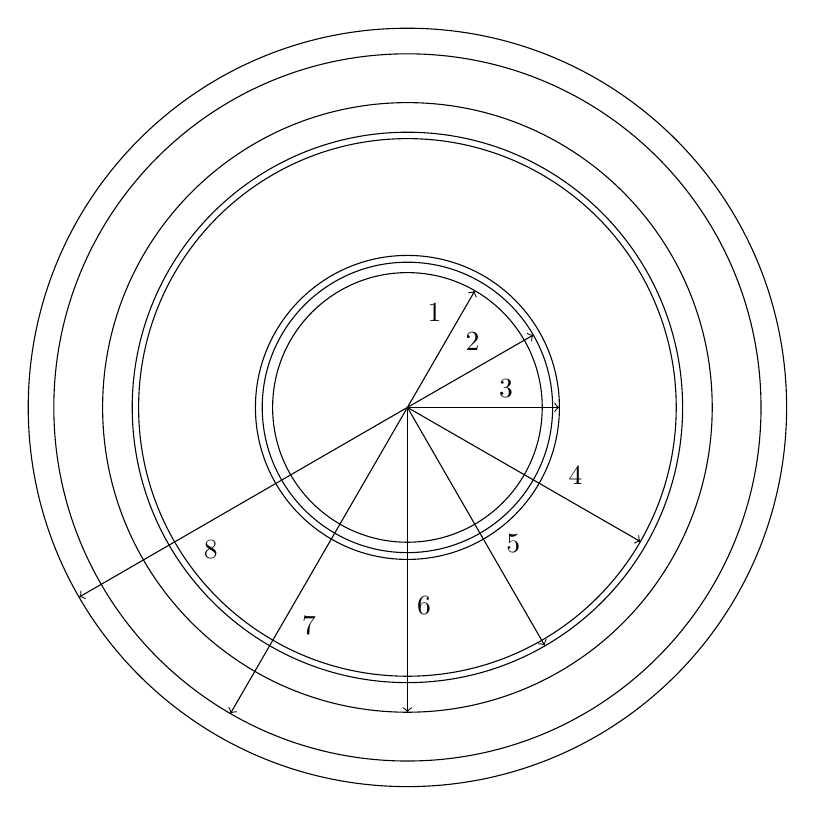
\begin{tikzpicture}[scale=8,auto]
        \draw (0,0) circle (0.214);
      \draw[->] (0,0) -- node[pos=0.65] {1} (0.107,0.185);
      \draw (0,0) circle (0.23051);
      \draw[->] (0,0) -- node[pos=0.65] {2} (0.2,0.115);
      \draw (0,0) circle (0.2413);
      \draw[->] (0,0) -- node[pos=0.65] {3} (0.241,0.0);
      \draw (0,0) circle (0.42672);
      \draw[->] (0,0) -- node[pos=0.65] {4} (0.37,-0.213);
      \draw (0,0) circle (0.43688);
      \draw[->] (0,0) -- node[pos=0.65] {5} (0.218,-0.378);
      \draw (0,0) circle (0.48387);
      \draw[->] (0,0) -- node[pos=0.65] {6} (0.0,-0.484);
      \draw (0,0) circle (0.56134);
      \draw[->] (0,0) -- node[pos=0.65] {7} (-0.281,-0.486);
      \draw (0,0) circle (0.60198);
      \draw[->] (0,0) -- node[pos=0.65] {8} (-0.521,-0.301);

      \end{tikzpicture}
      \begin{tikzpicture}
       \matrix [matrix of nodes]
      {
          Arrow & Radius (cm) & Material & \numrefheader \\
        1 & 0.21400 & \node[hyperlink node=mat_air]{Air}; & \ref{num:BPinnercladIR}\\ 
        2 & 0.23051 & \node[hyperlink node=mat_SS304]{SS304}; & \ref{num:BPinnercladOR}\\ 
        3 & 0.24130 & \node[hyperlink node=mat_helium]{Helium}; & \ref{num:BPpoisonIR}\\ 
        4 & 0.42672 & \node[hyperlink node=mat_borosilicate]{Borosilicate Glass}; & \ref{num:BPpoisonOR}\\ 
        5 & 0.43688 & \node[hyperlink node=mat_helium]{Helium}; & \ref{num:BPoutercladIR}\\ 
        6 & 0.48387 & \node[hyperlink node=mat_SS304]{SS304}; & \ref{num:BPoutercladOR}\\ 
        7 & 0.56134 & \node[hyperlink node=mat_water]{Water}; & \ref{num:GTIRrad}\\ 
        8 & 0.60198 & \node[hyperlink node=mat_zirc]{Zircaloy}; & \ref{num:GTORrad}\\ 
      };
\end{tikzpicture}
\end{geoitem}
\begin{geoitem}{\acs{BP} Plenum Geometry}{fig_ba_pin_plenum}\centering
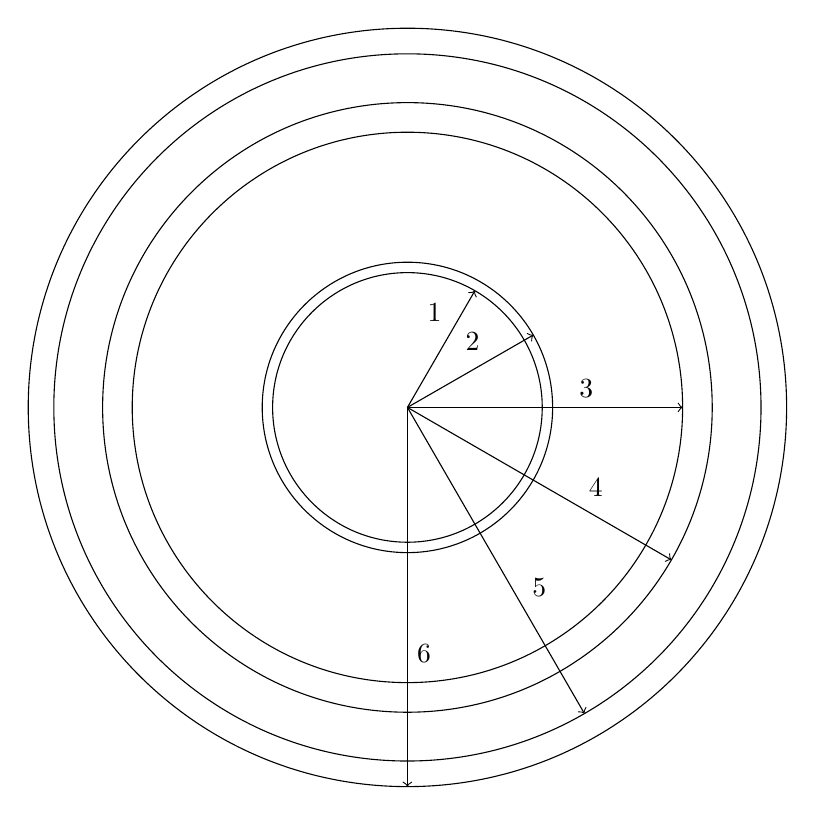
\begin{tikzpicture}[scale=8,auto]
        \draw (0,0) circle (0.214);
      \draw[->] (0,0) -- node[pos=0.65] {1} (0.107,0.185);
      \draw (0,0) circle (0.23051);
      \draw[->] (0,0) -- node[pos=0.65] {2} (0.2,0.115);
      \draw (0,0) circle (0.43688);
      \draw[->] (0,0) -- node[pos=0.65] {3} (0.437,0.0);
      \draw (0,0) circle (0.48387);
      \draw[->] (0,0) -- node[pos=0.65] {4} (0.419,-0.242);
      \draw (0,0) circle (0.56134);
      \draw[->] (0,0) -- node[pos=0.65] {5} (0.281,-0.486);
      \draw (0,0) circle (0.60198);
      \draw[->] (0,0) -- node[pos=0.65] {6} (0.0,-0.602);

      \end{tikzpicture}
      \begin{tikzpicture}
       \matrix [matrix of nodes]
      {
          Arrow & Radius (cm) & Material & \numrefheader \\
        1 & 0.21400 & \node[hyperlink node=mat_air]{Air}; & \ref{num:BPinnercladIR}\\ 
        2 & 0.23051 & \node[hyperlink node=mat_SS304]{SS304}; & \ref{num:BPinnercladOR}\\ 
        3 & 0.43688 & \node[hyperlink node=mat_helium]{Helium}; & \ref{num:BPoutercladIR}\\ 
        4 & 0.48387 & \node[hyperlink node=mat_SS304]{SS304}; & \ref{num:BPoutercladOR}\\ 
        5 & 0.56134 & \node[hyperlink node=mat_water]{Water}; & \ref{num:GTIRrad}\\ 
        6 & 0.60198 & \node[hyperlink node=mat_zirc]{Zircaloy}; & \ref{num:GTORrad}\\ 
      };
\end{tikzpicture}
\end{geoitem}
 % label: fig_ba_axials

%%%%%%%%%%%%%%%%%%%%%%%%%%%%%%%%%%%%%%%%%%%%%%%%%%%%%%%%%%%%%%%%%%%%%%%%%%%%%%%%
\subsubsection{Control Rods}
\label{sec:axial_cr}

Figure \ref{fig_cr_axials} shows the control rod axial layout, which depending
on the degree of insertion can either be occupied by the empty guide tube
pincell or the control rod pincell described in Section \ref{sec:pintypes}. The
details of insertion depend on the radial location of the specific control rod
cluster, i.e. which control or shutdown bank it belongs to. Unlike the other
axial descriptions in this section, Figure~\ref{fig_cr_axials} presents the
axial sections \emph{only} for the control rod thimble that fits inside the
guide tube. It is presented for the fully-inserted position; all intermediate
planes should be shifted according to the number of steps withdrawn, and the
appropriate axial sections created in combination with the surrounding guide
tube and grid spacer pincell.

In this model, when fully-inserted the top of the upper control rod active
absorber region should be flush with the top of the active fuel region. Control
rods are considered to be withdrawn in 228 "steps" until the active region is
drawn completely out of the active fuel region. When withdrawn 228 steps, the
bottom of the lower control rod active absorber region should be flush with the
top of the active fuel region. The total height of the lower and upper control
rod regions is 360.68 cm, meaning the step height is 1.58193 cm.

The actual axial planes used depend on the the number of steps of insertion of
the rod, and may be superseded by the highest axial plane when appropriate. In
other words, the planes presented in Figure~\ref{fig_cr_axials} should be
shifted upwards by the number of steps withdrawn times the step height.

The control and shutdown banks can have any level of partial insertion, where
the bottom tips of the rods can be at any axial step level between step 0 and
step 228. While each of these banks move their control rod clusters together,
their movement is often staggered with the other control rod banks, described in
Figure \ref{fig_cr_algorithm} with an insertion sequence example. However,
insertion levels for each individual bank are provided for most of the data
presented in this benchmark, so the algorithm in Figure \ref{fig_cr_algorithm}
may not be needed.

\begin{geoitem}{Control Rod Pin Upper Geometry}{fig_cr_pin_upper}\centering
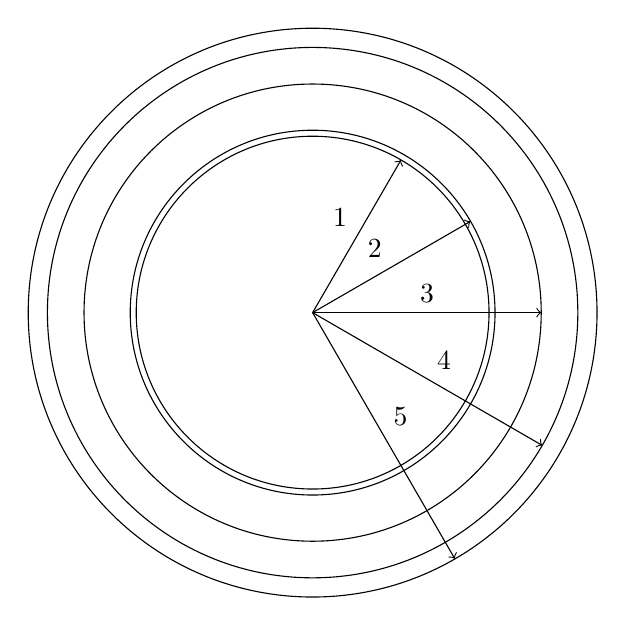
\begin{tikzpicture}[scale=6,auto]
        \draw (0,0) circle (0.37338);
      \draw[->] (0,0) -- node[pos=0.5] {1} (0.187,0.323);
      \draw (0,0) circle (0.38608);
      \draw[->] (0,0) -- node[pos=0.5] {2} (0.334,0.193);
      \draw (0,0) circle (0.48387);
      \draw[->] (0,0) -- node[pos=0.5] {3} (0.484,0.0);
      \draw (0,0) circle (0.56134);
      \draw[->] (0,0) -- node[pos=0.5] {4} (0.486,-0.281);
      \draw (0,0) circle (0.60198);
      \draw[->] (0,0) -- node[pos=0.5] {5} (0.301,-0.521);

      \end{tikzpicture}
      \begin{tikzpicture}
       \matrix [matrix of nodes]
      {
          Arrow & Radius (cm) & Material & \numrefheader \\
        1 & 0.37338 & \node[hyperlink node=mat_b4c_rod]{B4C}; & \ref{num:CRb4cOR}\\ 
        2 & 0.38608 & \node[hyperlink node=mat_helium]{Helium}; & \ref{num:CRthimIR}\\ 
        3 & 0.48387 & \node[hyperlink node=mat_SS304]{SS304}; & \ref{num:CRthimOR}\\ 
        4 & 0.56134 & \node[hyperlink node=mat_water]{Water}; & \ref{num:GTIRrad}\\ 
        5 & 0.60198 & \node[hyperlink node=mat_zirc]{Zircaloy}; & \ref{num:GTORrad}\\ 
      };
\end{tikzpicture}
\end{geoitem}
\begin{geoitem}{Control Rod Pin Lower Geometry}{fig_cr_pin}\centering
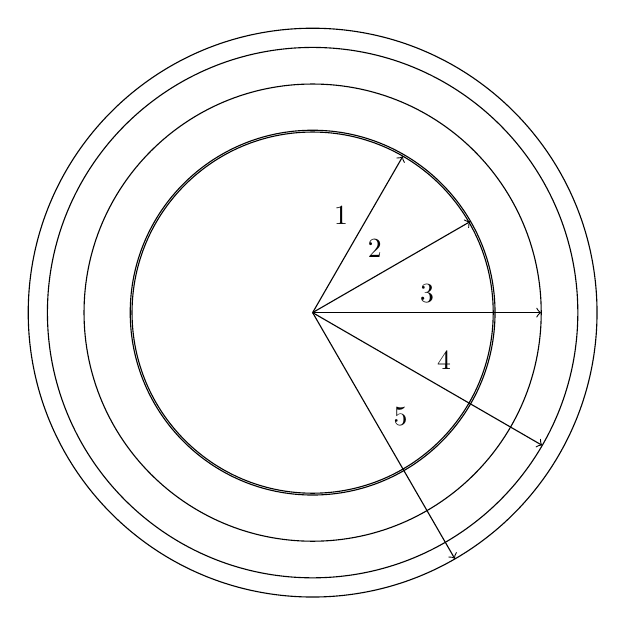
\begin{tikzpicture}[scale=6,auto]
        \draw (0,0) circle (0.38227);
      \draw[->] (0,0) -- node[pos=0.5] {1} (0.191,0.331);
      \draw (0,0) circle (0.38608);
      \draw[->] (0,0) -- node[pos=0.5] {2} (0.334,0.193);
      \draw (0,0) circle (0.48387);
      \draw[->] (0,0) -- node[pos=0.5] {3} (0.484,0.0);
      \draw (0,0) circle (0.56134);
      \draw[->] (0,0) -- node[pos=0.5] {4} (0.486,-0.281);
      \draw (0,0) circle (0.60198);
      \draw[->] (0,0) -- node[pos=0.5] {5} (0.301,-0.521);

      \end{tikzpicture}
      \begin{tikzpicture}
       \matrix [matrix of nodes]
      {
          Arrow & Radius (cm) & Material & \numrefheader \\
        1 & 0.38227 & \node[hyperlink node=mat_aic_rod]{Ag-In-Cd}; & \ref{num:CRaicOR}\\ 
        2 & 0.38608 & \node[hyperlink node=mat_helium]{Helium}; & \ref{num:CRthimIR}\\ 
        3 & 0.48387 & \node[hyperlink node=mat_SS304]{SS304}; & \ref{num:CRthimOR}\\ 
        4 & 0.56134 & \node[hyperlink node=mat_water]{Water}; & \ref{num:GTIRrad}\\ 
        5 & 0.60198 & \node[hyperlink node=mat_zirc]{Zircaloy}; & \ref{num:GTORrad}\\ 
      };
\end{tikzpicture}
\end{geoitem}
\begin{geoitem}{Control Rod Pin Spacer Geometry}{fig_cr_pin_spacer}\centering
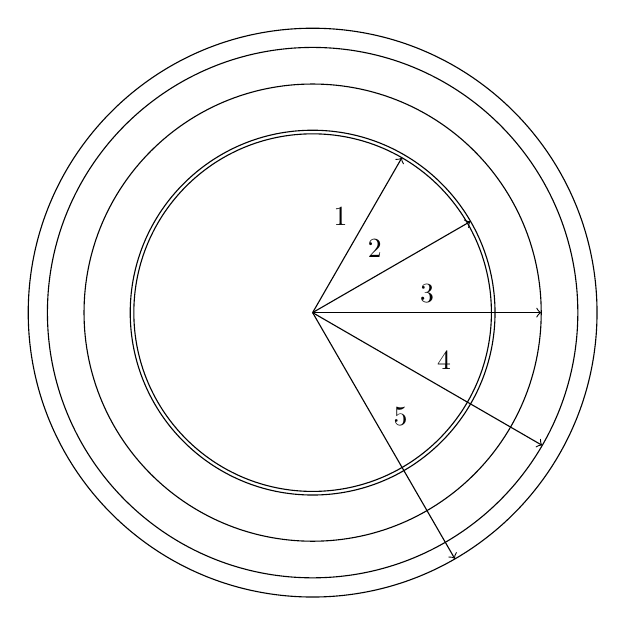
\begin{tikzpicture}[scale=6,auto]
        \draw (0,0) circle (0.37845);
      \draw[->] (0,0) -- node[pos=0.5] {1} (0.189,0.328);
      \draw (0,0) circle (0.38608);
      \draw[->] (0,0) -- node[pos=0.5] {2} (0.334,0.193);
      \draw (0,0) circle (0.48387);
      \draw[->] (0,0) -- node[pos=0.5] {3} (0.484,0.0);
      \draw (0,0) circle (0.56134);
      \draw[->] (0,0) -- node[pos=0.5] {4} (0.486,-0.281);
      \draw (0,0) circle (0.60198);
      \draw[->] (0,0) -- node[pos=0.5] {5} (0.301,-0.521);

      \end{tikzpicture}
      \begin{tikzpicture}
       \matrix [matrix of nodes]
      {
          Arrow & Radius (cm) & Material & \numrefheader \\
        1 & 0.37845 & \node[hyperlink node=mat_SS304]{SS304}; & \ref{num:CRspacerOR}\\ 
        2 & 0.38608 & \node[hyperlink node=mat_helium]{Helium}; & \ref{num:CRthimIR}\\ 
        3 & 0.48387 & \node[hyperlink node=mat_SS304]{SS304}; & \ref{num:CRthimOR}\\ 
        4 & 0.56134 & \node[hyperlink node=mat_water]{Water}; & \ref{num:GTIRrad}\\ 
        5 & 0.60198 & \node[hyperlink node=mat_zirc]{Zircaloy}; & \ref{num:GTORrad}\\ 
      };
\end{tikzpicture}
\end{geoitem}
\begin{geoitem}{Control Rod Pin Plenum Geometry}{fig_cr_pin_plenum}\centering
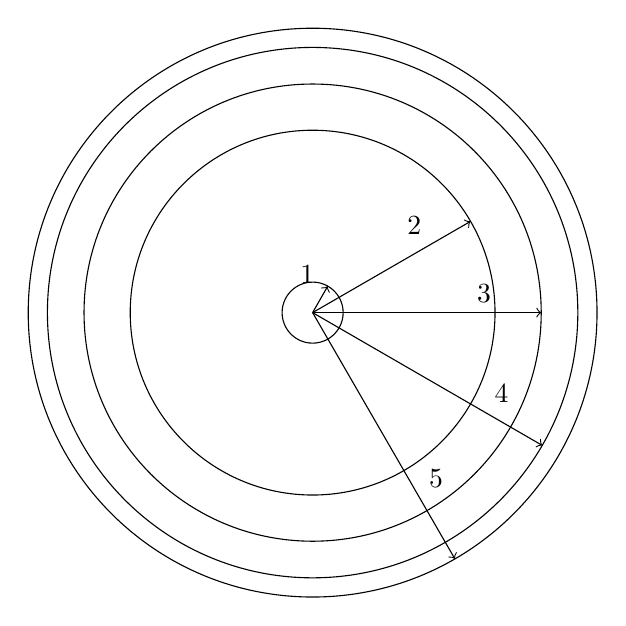
\begin{tikzpicture}[scale=6,auto]
        \draw (0,0) circle (0.06459);
      \draw[->] (0,0) -- node[pos=0.75] {1} (0.032,0.056);
      \draw (0,0) circle (0.38608);
      \draw[->] (0,0) -- node[pos=0.75] {2} (0.334,0.193);
      \draw (0,0) circle (0.48387);
      \draw[->] (0,0) -- node[pos=0.75] {3} (0.484,0.0);
      \draw (0,0) circle (0.56134);
      \draw[->] (0,0) -- node[pos=0.75] {4} (0.486,-0.281);
      \draw (0,0) circle (0.60198);
      \draw[->] (0,0) -- node[pos=0.75] {5} (0.301,-0.521);

      \end{tikzpicture}
      \begin{tikzpicture}
       \matrix [matrix of nodes]
      {
          Arrow & Radius (cm) & Material & \numrefheader \\
        1 & 0.06459 & \node[hyperlink node=mat_inconel]{Inconel}; & \ref{num:cr_plenum_spring}\\ 
        2 & 0.38608 & \node[hyperlink node=mat_helium]{Helium}; & \ref{num:CRthimIR}\\ 
        3 & 0.48387 & \node[hyperlink node=mat_SS304]{SS304}; & \ref{num:CRthimOR}\\ 
        4 & 0.56134 & \node[hyperlink node=mat_water]{Water}; & \ref{num:GTIRrad}\\ 
        5 & 0.60198 & \node[hyperlink node=mat_zirc]{Zircaloy}; & \ref{num:GTORrad}\\ 
      };
\end{tikzpicture}
\end{geoitem}
 % label: fig_cr_axials


\begin{figure}

  \centering
  \fbox{
    \begin{minipage}{6.5in}
      \textbf{Control Rod Insertion Sequence}
      ~\\
      ~\\
      Starting from all rods fully withdrawn:
      
      \begin{itemize}
        \item First D moves in alone, until it gets to 113 steps withdrawn
        \item Now D and C move together until C gets to 113 steps withdrawn \\(D is all the way in when C is at 115)
        \item Now C and B move together until B gets to 113 steps withdrawn \\(C is all the way in when B is at 115)
        \item Now B and A move together until A gets to 0 steps withdrawn \\(B is all the way in when A is at 115)
      \end{itemize}
      
      Assuming only movement of each control rod bank by one step at a time, in
      total this sequence yields 574 unique positions, which we denote with
      integer $\mathbb{S}$ steps withdrawn. If $\mathbb{S}=0$ all control rods
      are out of the core, and if $\mathbb{S}=574$ all rods are fully inserted.
      For example for normal operation with the D bank at the bite position of
      $\mathbb{S}_D = 213$ steps withdrawn, $\mathbb{S}=228-213=15$. With this
      notation, the following algorithm provides the elevation of the axial
      planes of the active region in each control rod bank ($s_i^{\mathrm{bot}}$
      and $s_i^{\mathrm{top}}$) for a given $\mathbb{S}$ with the fully inserted
      elevation $s_0$ and step width $\delta$.

      \begin{align*}
        \mathbb{S}_D &=  \max(0,~228-\mathbb{S}) \\
        \mathbb{S}_C &=  (\mathbb{S}_D<113) ~?~ \max(0,~228-\mathbb{S}+113  +3) ~:~ 228 \\
        \mathbb{S}_B &=  (\mathbb{S}_C<113) ~?~ \max(0,~228-\mathbb{S}+113\times 2+5) ~:~ 228 \\
        \mathbb{S}_A &=  (\mathbb{S}_B<113) ~?~ \max(0,~228-\mathbb{S}+113\times 3+7) ~:~ 228 \\
\\
        s_A^{\mathrm{bot}} &=  s_0 + \delta \times \mathbb{S}_A \\
        s_B^{\mathrm{bot}} &=  s_0 + \delta \times \mathbb{S}_B \\
        s_C^{\mathrm{bot}} &=  s_0 + \delta \times \mathbb{S}_C \\
        s_D^{\mathrm{bot}} &=  s_0 + \delta \times \mathbb{S}_D \\
\\
        s_A^{\mathrm{top}} &=  s_A^{\mathrm{bot}} + \delta \times 228 \\
        s_B^{\mathrm{top}} &=  s_B^{\mathrm{bot}} + \delta \times 228 \\
        s_C^{\mathrm{top}} &=  s_C^{\mathrm{bot}} + \delta \times 228 \\
        s_D^{\mathrm{top}} &=  s_D^{\mathrm{bot}} + \delta \times 228 \\
      \end{align*}
      
    \end{minipage}
  }
  
  \caption[Control rod insertion sequence and axial specification]{ Control rod insertion sequence and axial specification \cite{smith_comm}. \label{fig_cr_algorithm}}

\end{figure}


%%%%%%%%%%%%%%%%%%%%%%%%%%%%%%%%%%%%%%%%%%%%%%%%%%%%%%%%%%%%%%%%%%%%%%%%%%%%%%%%
\subsubsection{Aggregate}

By defining the full extent of the axial geometry in the pincells, several
features remain to be described or examined in the final combination of each
element of the model. In aggregate it is useful to see an exhaustive list of
all axial planes used in the model, as presented in Figure \ref{fig_all_axials}.
Control rod insertions are treated separately, as discussed in Section
\ref{sec:axial_cr}.

\begin{figure}[htbp]
    \centering
    \begin{tikzpicture}[scale=1,x=1in,y=1in]
      \draw[white] (-2.0,-2.0) rectangle (2.0,2.0);
      \node {\pgftext{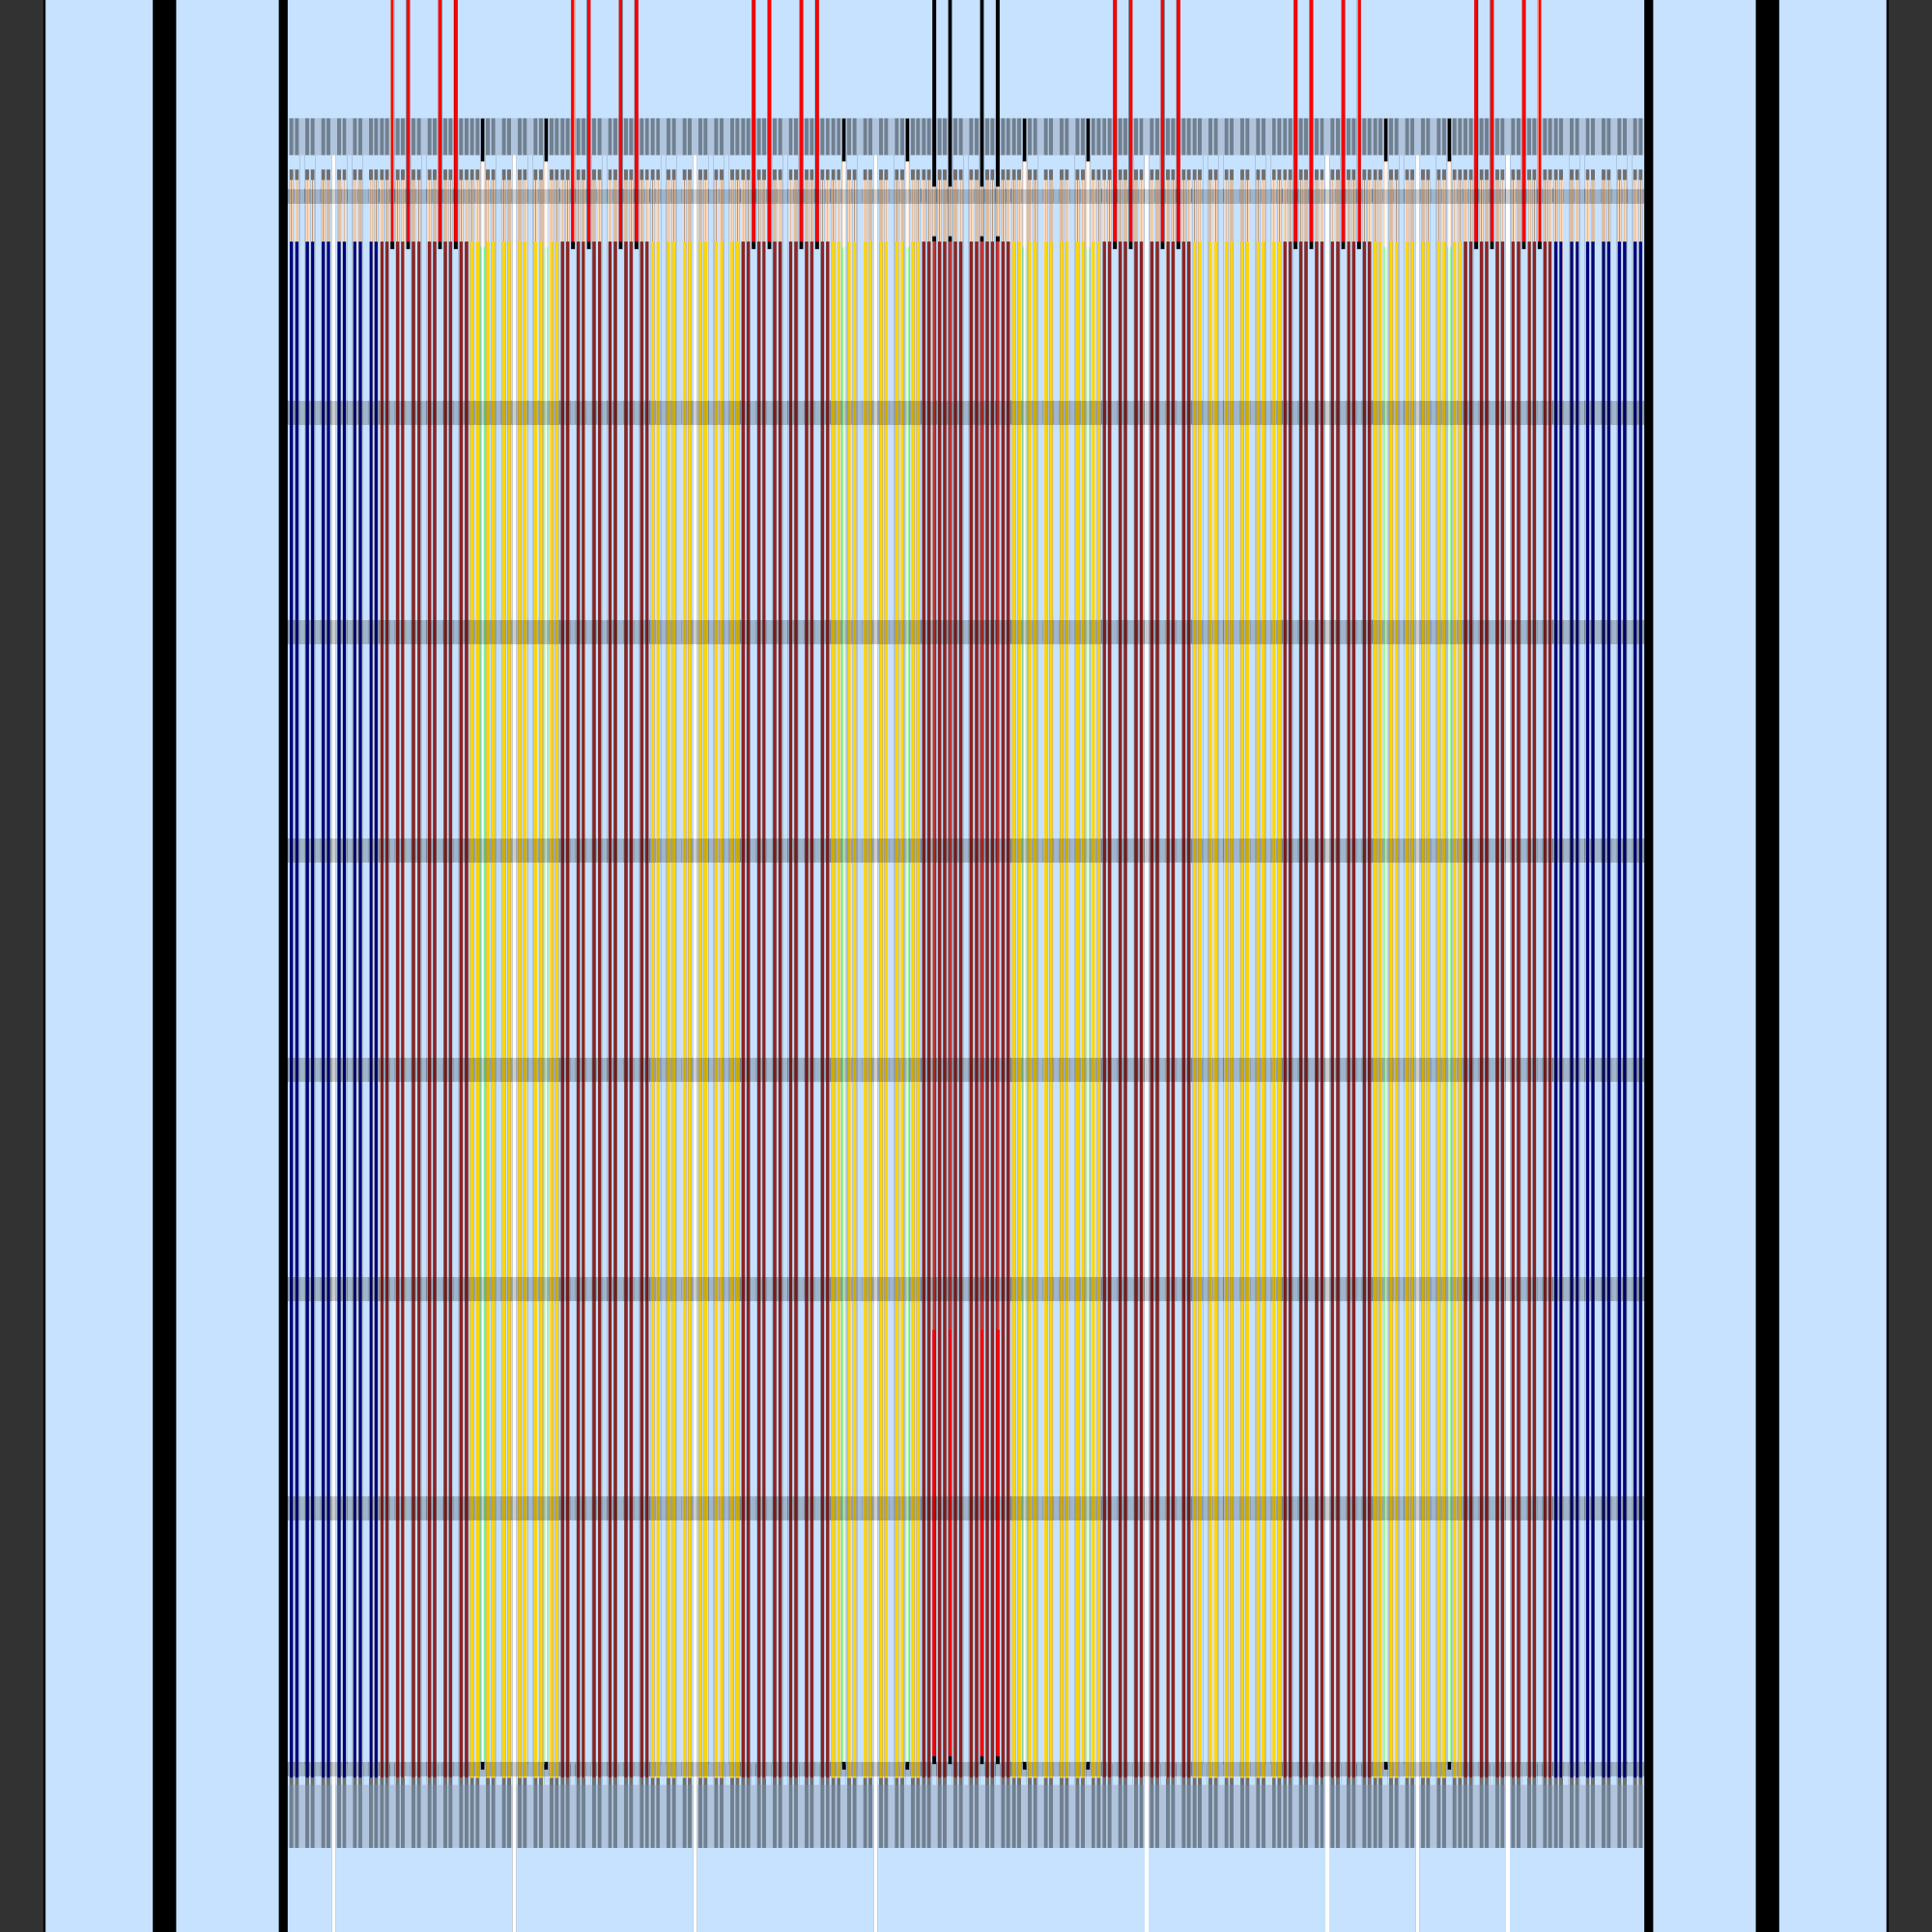
\includegraphics[width=4.0in]{specifications/axial/figs/row_8_mats_axial_grids_enhanced.png}}};
      \draw[red] (1.40241130435,-2.0) -- (2.2,-2.0) -- (2.4,-2.0) -- (2.55,-2.0) node[black,right,anchor=west,font=\scriptsize] {~0.00000 ~~~~~~~~ Lowest Extent};
      \draw[red] (1.40241130435,-1.82608695652) -- (2.2,-1.82608695652) -- (2.4,-1.88235294118) -- (2.55,-1.88235294118) node[black,right,anchor=west,font=\scriptsize] {~20.0000 ~~~~~~~~ Bottom of Support Plate};
      \draw[red] (1.40241130435,-1.69565217391) -- (2.2,-1.69565217391) -- (2.4,-1.76470588235) -- (2.55,-1.76470588235) node[black,right,anchor=west,font=\scriptsize] {~35.0000 ~~~~~~~~ Bottom of Fuel Rod};
      \draw[red] (1.40241130435,-1.68045217391) -- (2.2,-1.68045217391) -- (2.4,-1.64705882353) -- (2.55,-1.64705882353) node[black,right,anchor=west,font=\scriptsize] {~36.7480 ~~~~~~~~ Bottom of Active Fuel};
      \draw[red] (1.40241130435,-1.67685130435) -- (2.2,-1.67685130435) -- (2.4,-1.52941176471) -- (2.55,-1.52941176471) node[black,right,anchor=west,font=\scriptsize] {~37.1621 ~~~~~~~~ Grid 1 Bottom};
      \draw[red] (1.40241130435,-1.66382608696) -- (2.2,-1.66382608696) -- (2.4,-1.41176470588) -- (2.55,-1.41176470588) node[black,right,anchor=west,font=\scriptsize] {~38.6600 ~~~~~~~~ Bot. of BPRA Rod};
      \draw[red] (1.40241130435,-1.65253913043) -- (2.2,-1.65253913043) -- (2.4,-1.29411764706) -- (2.55,-1.29411764706) node[black,right,anchor=west,font=\scriptsize] {~39.9580 ~~~~~~~~ Control Rod Step 0};
      \draw[red] (1.40241130435,-1.64765217391) -- (2.2,-1.64765217391) -- (2.4,-1.17647058824) -- (2.55,-1.17647058824) node[black,right,anchor=west,font=\scriptsize] {~40.5200 ~~~~~~~~ Grid 1 Top};
      \draw[red] (1.40241130435,-1.64732173913) -- (2.2,-1.64732173913) -- (2.4,-1.05882352941) -- (2.55,-1.05882352941) node[black,right,anchor=west,font=\scriptsize] {~40.5580 ~~~~~~~~ Bottom of Active Absorber};
      \draw[red] (1.40241130435,-1.63627826087) -- (2.2,-1.63627826087) -- (2.4,-0.941176470588) -- (2.55,-0.941176470588) node[black,right,anchor=west,font=\scriptsize] {~41.8280 ~~~~~~~~ Bottom of Lower Absorber (AIC)};
      \draw[red] (1.40241130435,-1.14760869565) -- (2.2,-1.14760869565) -- (2.4,-0.823529411765) -- (2.55,-0.823529411765) node[black,right,anchor=west,font=\scriptsize] {~98.0250 ~~~~~~~~ Grid 2 Bottom};
      \draw[red] (1.40241130435,-1.09791304348) -- (2.2,-1.09791304348) -- (2.4,-0.705882352941) -- (2.55,-0.705882352941) node[black,right,anchor=west,font=\scriptsize] {~103.740 ~~~~~~~~ Grid 2 Top};
      \draw[red] (1.40241130435,-0.69372173913) -- (2.2,-0.69372173913) -- (2.4,-0.588235294118) -- (2.55,-0.588235294118) node[black,right,anchor=west,font=\scriptsize] {~150.222 ~~~~~~~~ Grid 3 Bottom};
      \draw[red] (1.40241130435,-0.644026086957) -- (2.2,-0.644026086957) -- (2.4,-0.470588235294) -- (2.55,-0.470588235294) node[black,right,anchor=west,font=\scriptsize] {~155.937 ~~~~~~~~ Grid 3 Top};
      \draw[red] (1.40241130435,-0.239834782609) -- (2.2,-0.239834782609) -- (2.4,-0.352941176471) -- (2.55,-0.352941176471) node[black,right,anchor=west,font=\scriptsize] {~202.419 ~~~~~~~~ Grid 4 Bottom};
      \draw[red] (1.40241130435,-0.190139130435) -- (2.2,-0.190139130435) -- (2.4,-0.235294117647) -- (2.55,-0.235294117647) node[black,right,anchor=west,font=\scriptsize] {~208.134 ~~~~~~~~ Grid 4 Top};
      \draw[red] (1.40241130435,0.214052173913) -- (2.2,0.214052173913) -- (2.4,-0.117647058824) -- (2.55,-0.117647058824) node[black,right,anchor=west,font=\scriptsize] {~254.616 ~~~~~~~~ Grid 5 Bottom};
      \draw[red] (1.40241130435,0.263747826087) -- (2.2,0.263747826087) -- (2.4,0.0) -- (2.55,0.0) node[black,right,anchor=west,font=\scriptsize] {~260.331 ~~~~~~~~ Grid 5 Top};
      \draw[red] (1.40241130435,0.667939130435) -- (2.2,0.667939130435) -- (2.4,0.117647058824) -- (2.55,0.117647058824) node[black,right,anchor=west,font=\scriptsize] {~306.813 ~~~~~~~~ Grid 6 Bottom};
      \draw[red] (1.40241130435,0.717634782609) -- (2.2,0.717634782609) -- (2.4,0.235294117647) -- (2.55,0.235294117647) node[black,right,anchor=west,font=\scriptsize] {~312.528 ~~~~~~~~ Grid 6 Top};
      \draw[red] (1.40241130435,1.12182608696) -- (2.2,1.12182608696) -- (2.4,0.352941176471) -- (2.55,0.352941176471) node[black,right,anchor=west,font=\scriptsize] {~359.010 ~~~~~~~~ Grid 7 Bottom};
      \draw[red] (1.40241130435,1.17152173913) -- (2.2,1.17152173913) -- (2.4,0.470588235294) -- (2.55,0.470588235294) node[black,right,anchor=west,font=\scriptsize] {~364.725 ~~~~~~~~ Grid 7 Top};
      \draw[red] (1.40241130435,1.48380869565) -- (2.2,1.48380869565) -- (2.4,0.588235294118) -- (2.55,0.588235294118) node[black,right,anchor=west,font=\scriptsize] {~400.638 ~~~~~~~~ Control Rod Step 228};
      \draw[red] (1.40241130435,1.48902608696) -- (2.2,1.48902608696) -- (2.4,0.705882352941) -- (2.55,0.705882352941) node[black,right,anchor=west,font=\scriptsize] {~401.238 ~~~~~~~~ Top of Active Absorber};
      \draw[red] (1.40241130435,1.50006956522) -- (2.2,1.50006956522) -- (2.4,0.823529411765) -- (2.55,0.823529411765) node[black,right,anchor=west,font=\scriptsize] {~402.508 ~~~~~~~~ Top of Active Fuel};
      \draw[red] (1.40241130435,1.51111304348) -- (2.2,1.51111304348) -- (2.4,0.941176470588) -- (2.55,0.941176470588) node[black,right,anchor=west,font=\scriptsize] {~403.778 ~~~~~~~~ Bottom of Control Rod Plenum};
      \draw[red] (1.40241130435,1.58092173913) -- (2.2,1.58092173913) -- (2.4,1.05882352941) -- (2.55,1.05882352941) node[black,right,anchor=west,font=\scriptsize] {~411.806 ~~~~~~~~ Grid 8 Bottom};
      \draw[red] (1.40241130435,1.61012173913) -- (2.2,1.61012173913) -- (2.4,1.17647058824) -- (2.55,1.17647058824) node[black,right,anchor=west,font=\scriptsize] {~415.164 ~~~~~~~~ Grid 8 Top};
      \draw[red] (1.40241130435,1.61354782609) -- (2.2,1.61354782609) -- (2.4,1.29411764706) -- (2.55,1.29411764706) node[black,right,anchor=west,font=\scriptsize] {~415.558 ~~~~~~~~ Top of Control Rod Plenum};
      \draw[red] (1.40241130435,1.62751304348) -- (2.2,1.62751304348) -- (2.4,1.41176470588) -- (2.55,1.41176470588) node[black,right,anchor=west,font=\scriptsize] {~417.164 ~~~~~~~~ Top of Fuel Rod Plenum};
      \draw[red] (1.40241130435,1.6496) -- (2.2,1.6496) -- (2.4,1.52941176471) -- (2.55,1.52941176471) node[black,right,anchor=west,font=\scriptsize] {~419.704 ~~~~~~~~ Top of Fuel Rod};
      \draw[red] (1.40241130435,1.66549565217) -- (2.2,1.66549565217) -- (2.4,1.64705882353) -- (2.55,1.64705882353) node[black,right,anchor=west,font=\scriptsize] {~421.532 ~~~~~~~~ Top of BPRA Rod Plenum};
      \draw[red] (1.40241130435,1.67868695652) -- (2.2,1.67868695652) -- (2.4,1.76470588235) -- (2.55,1.76470588235) node[black,right,anchor=west,font=\scriptsize] {~423.049 ~~~~~~~~ Bottom of Upper Nozzle};
      \draw[red] (1.40241130435,1.75544347826) -- (2.2,1.75544347826) -- (2.4,1.88235294118) -- (2.55,1.88235294118) node[black,right,anchor=west,font=\scriptsize] {~431.876 ~~~~~~~~ Top of Upper Nozzle};
      \draw[red] (1.40241130435,2.0) -- (2.2,2.0) -- (2.4,2.0) -- (2.55,2.0) node[black,right,anchor=west,font=\scriptsize] {~460.000 ~~~~~~~~ Highest Extent};
      \draw (2.4,2.11764705882) node[left,anchor=west,font=\scriptsize] {\underline{Elevation (cm)} ~~~ \underline{Description}};

    \end{tikzpicture}


    \caption[Scale view of all axial planes.]{\emph{Left}: Scale view of row 8 axial cross section, with highlighted grid spacers and partial insertion of control rod bank D to the bite position. \emph{Right}: exhaustive list of all axial planes used in the model, excluding partial control rod insertion planes.\label{fig_all_axials}}
\end{figure} % label: fig_all_axials

\paragraph{Grid Spacers}

Nearly all axial features of the model are captured in the axial pincell
specifications. However, the stainless steel grid sleeve described in Section
\ref{sec:rad_grids} for each of the 8 grid spacers needs to be defined on the
assembly level, as it is not contained within any of the pincell elements.  The
axial planes used for the grid sleeves are the same as those used for the grids
in the pincells, as listed in Figure \ref{fig_all_axials}.

\paragraph{Nozzles and Support Plate}\label{par:nozzle}

By defining pincells as solid material pins below and
above the fuel rod regions, the model implicitly approximates the nozzle and
support plate regions as depicted in Figure \ref{fig_nozzles}.  While the axial
planes used here were taken from Source \ref{num:watts_bar}, this does not
necessarily represent the true geometry of this portion of the reactor.  However,
the special densities of water and steel for the nozzle sections were
calculated such that the mass and volume fractions of the materials are
consistent with \cite{ml033530020}. The material compositions of borated water 
and steel in the nozzle and support plate are in Material \ref{mat_water_spn}
and Material \ref{mat_ss_spn} respectively.
Thus, when modeling, the material "Nozzle / Support Plate Stainless Steel"
(\ref{mat_ss_spn}) rather than "Stainless Steel" should be used for all the fuel
rods in the upper and lower nozzle / support plate regions as depicted in Figure
\ref{fig_fuel_axials}, while the material "Nozzle / Support Plate Borated Water"
(\ref{mat_ss_spn}) rather than "Borated Water" should be used for the water in
the nozzles and support plate (Figure \ref{fig_gtu_axials}). Figures
\ref{fig_fuel_axials} through \ref{fig:tb_detail} illustrate the modeling details
with material names and colors that preserve the actual masses of material. 
Note that since the bottom nozzle and
support plate are both stainless steel, no distinction is made between the two
regions.

\begin{figure}[htpb]
  \centering
  
\includegraphics[width=3in]{specifications/axial/figs/J8_nozzle.png}
  \caption{Radial picture of nozzles and support plate in aggregate model \label{fig_nozzles}}
\end{figure}

\paragraph{Top and Bottom of the Core}

For verification, Figure \ref{fig:tb_detail} shows scale
views close to the bottom and top regions of the core resulting from the
aggregate pincell specification as defined previously.

\begin{figure}[h]
    \centering
    \begin{tikzpicture}[x=1cm,y=1cm]
      \def\height{9}
      
      \draw[white] (-\height/2,\height/2) rectangle (\height*1.1,-\height*1.5);
      
      \node (toppic) at (0,0) {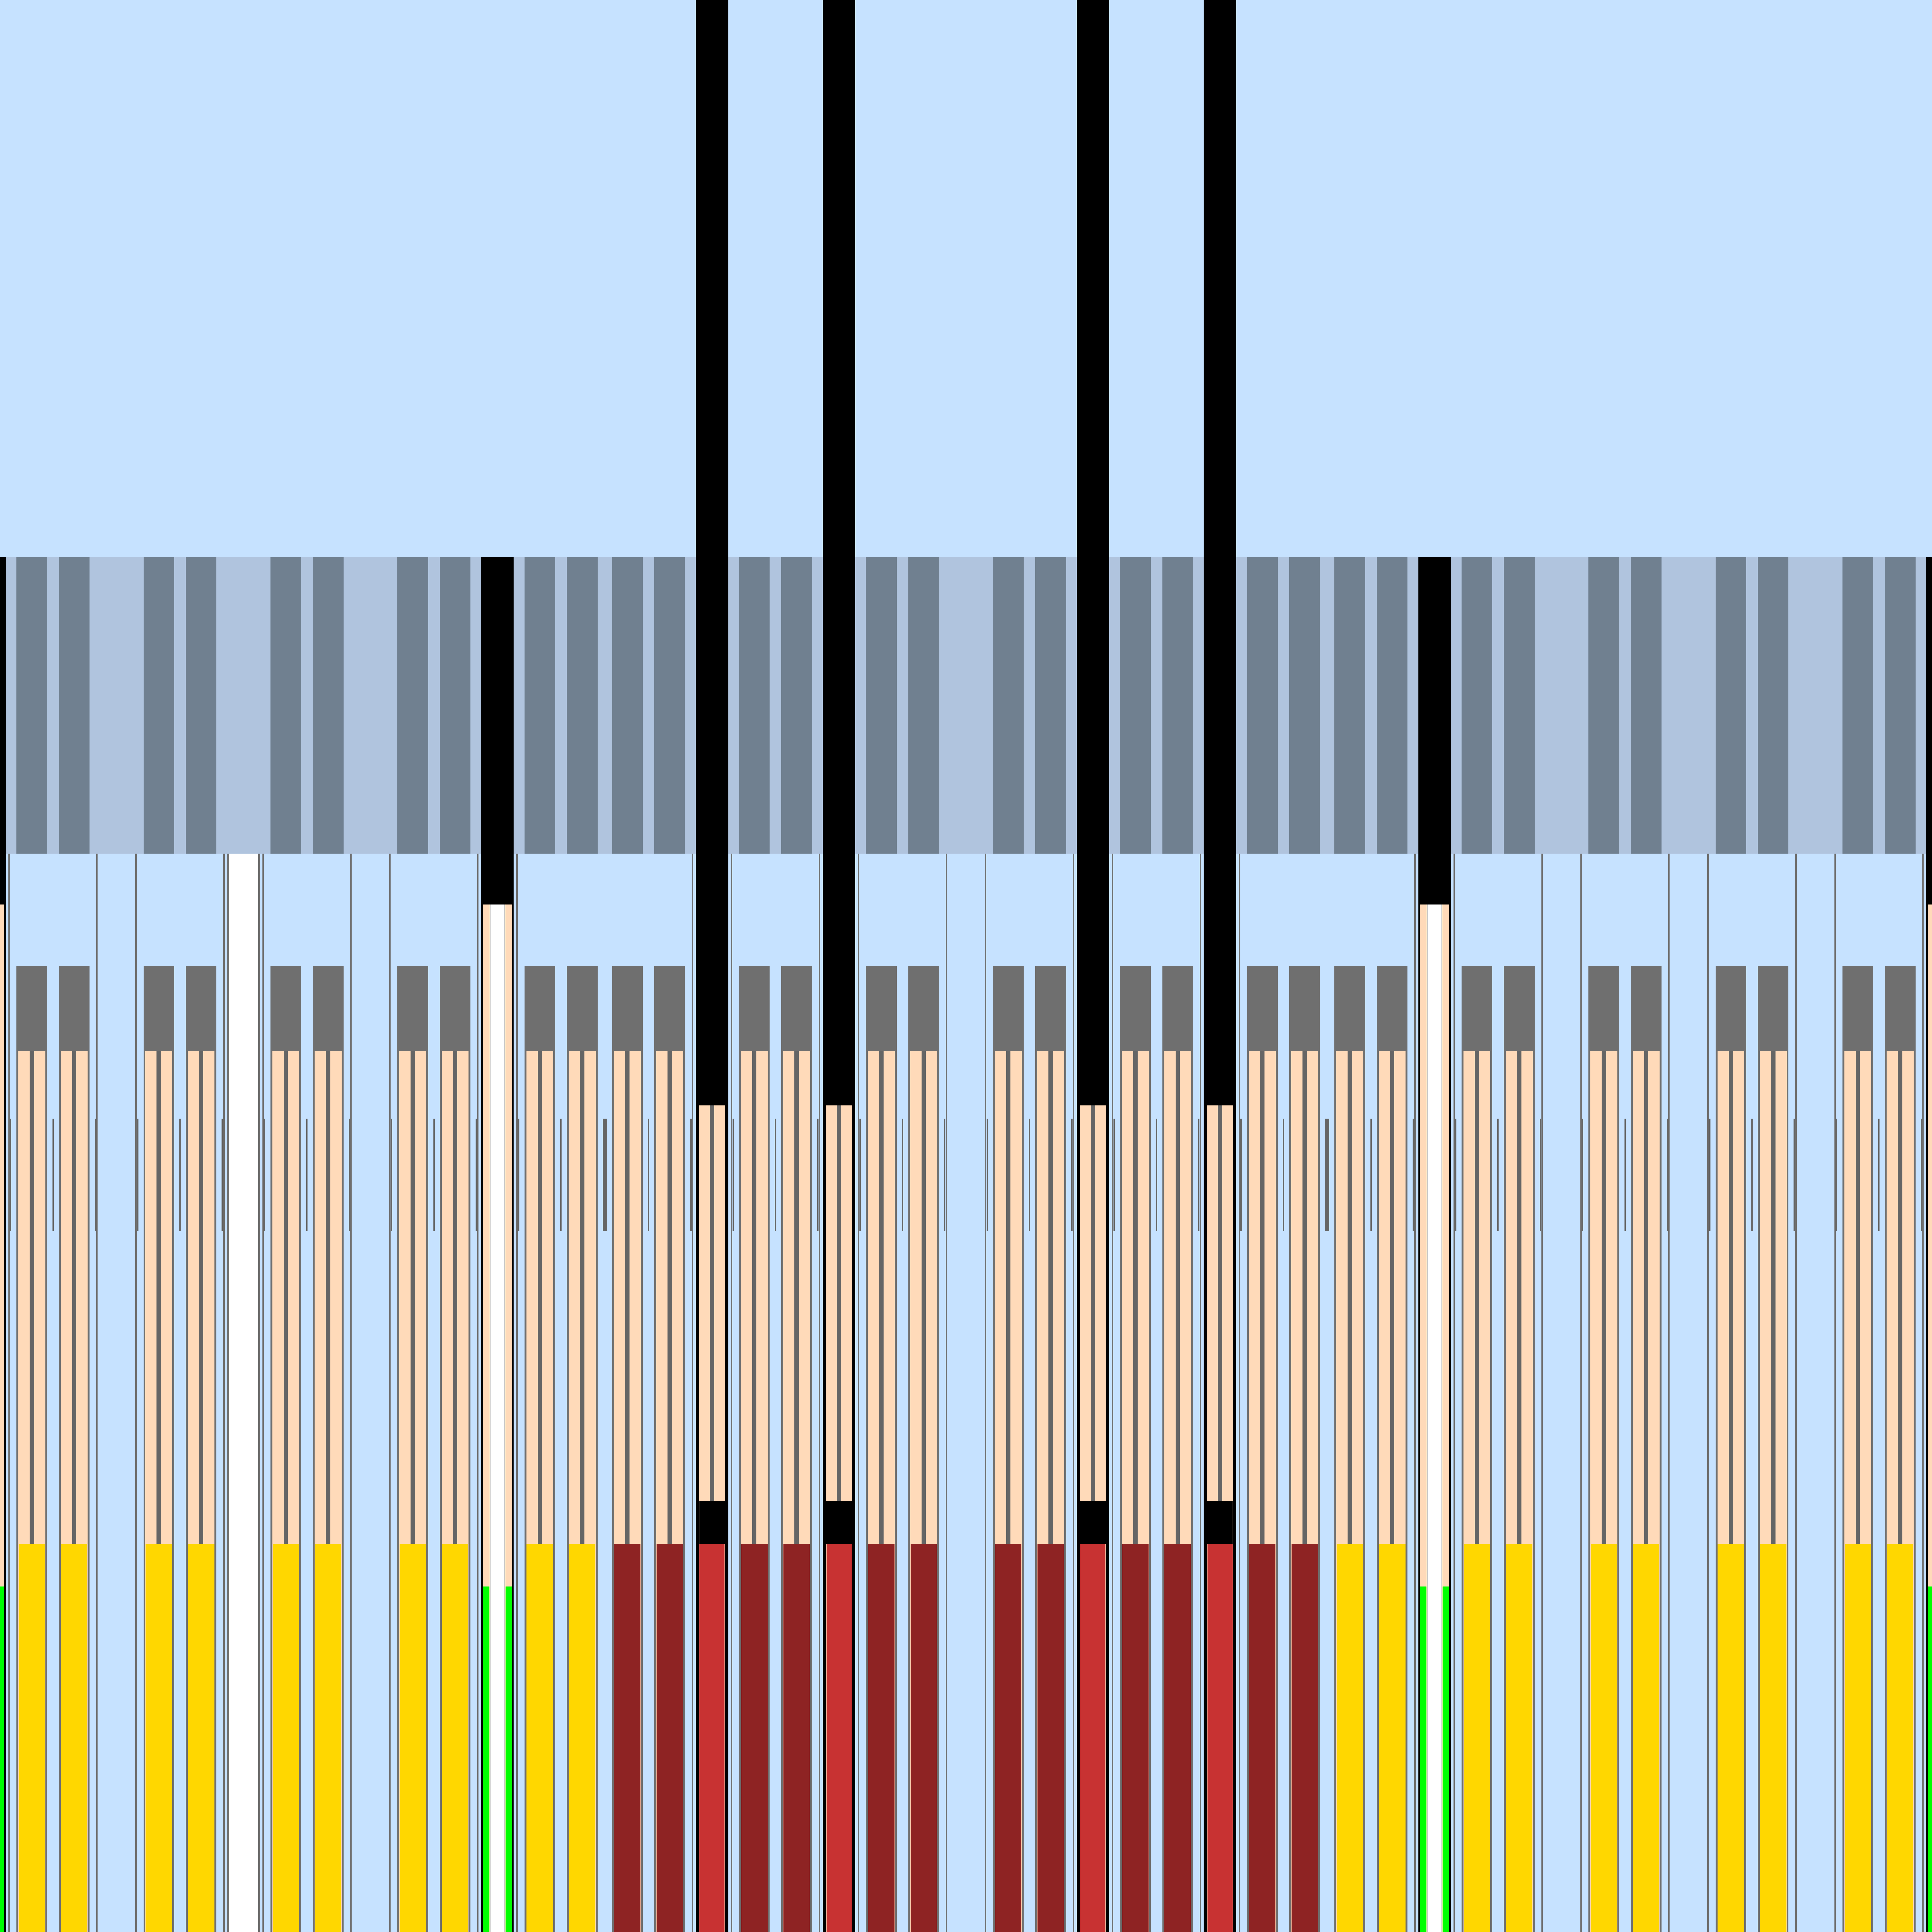
\includegraphics[height=\height cm]{specifications/axial/figs/axial_mats_row_8_topzoom.png}};
      \node[anchor=north] (dots) at (toppic.south) {$\vdots$};
      \node[anchor=north] (botpic) at (dots.south) {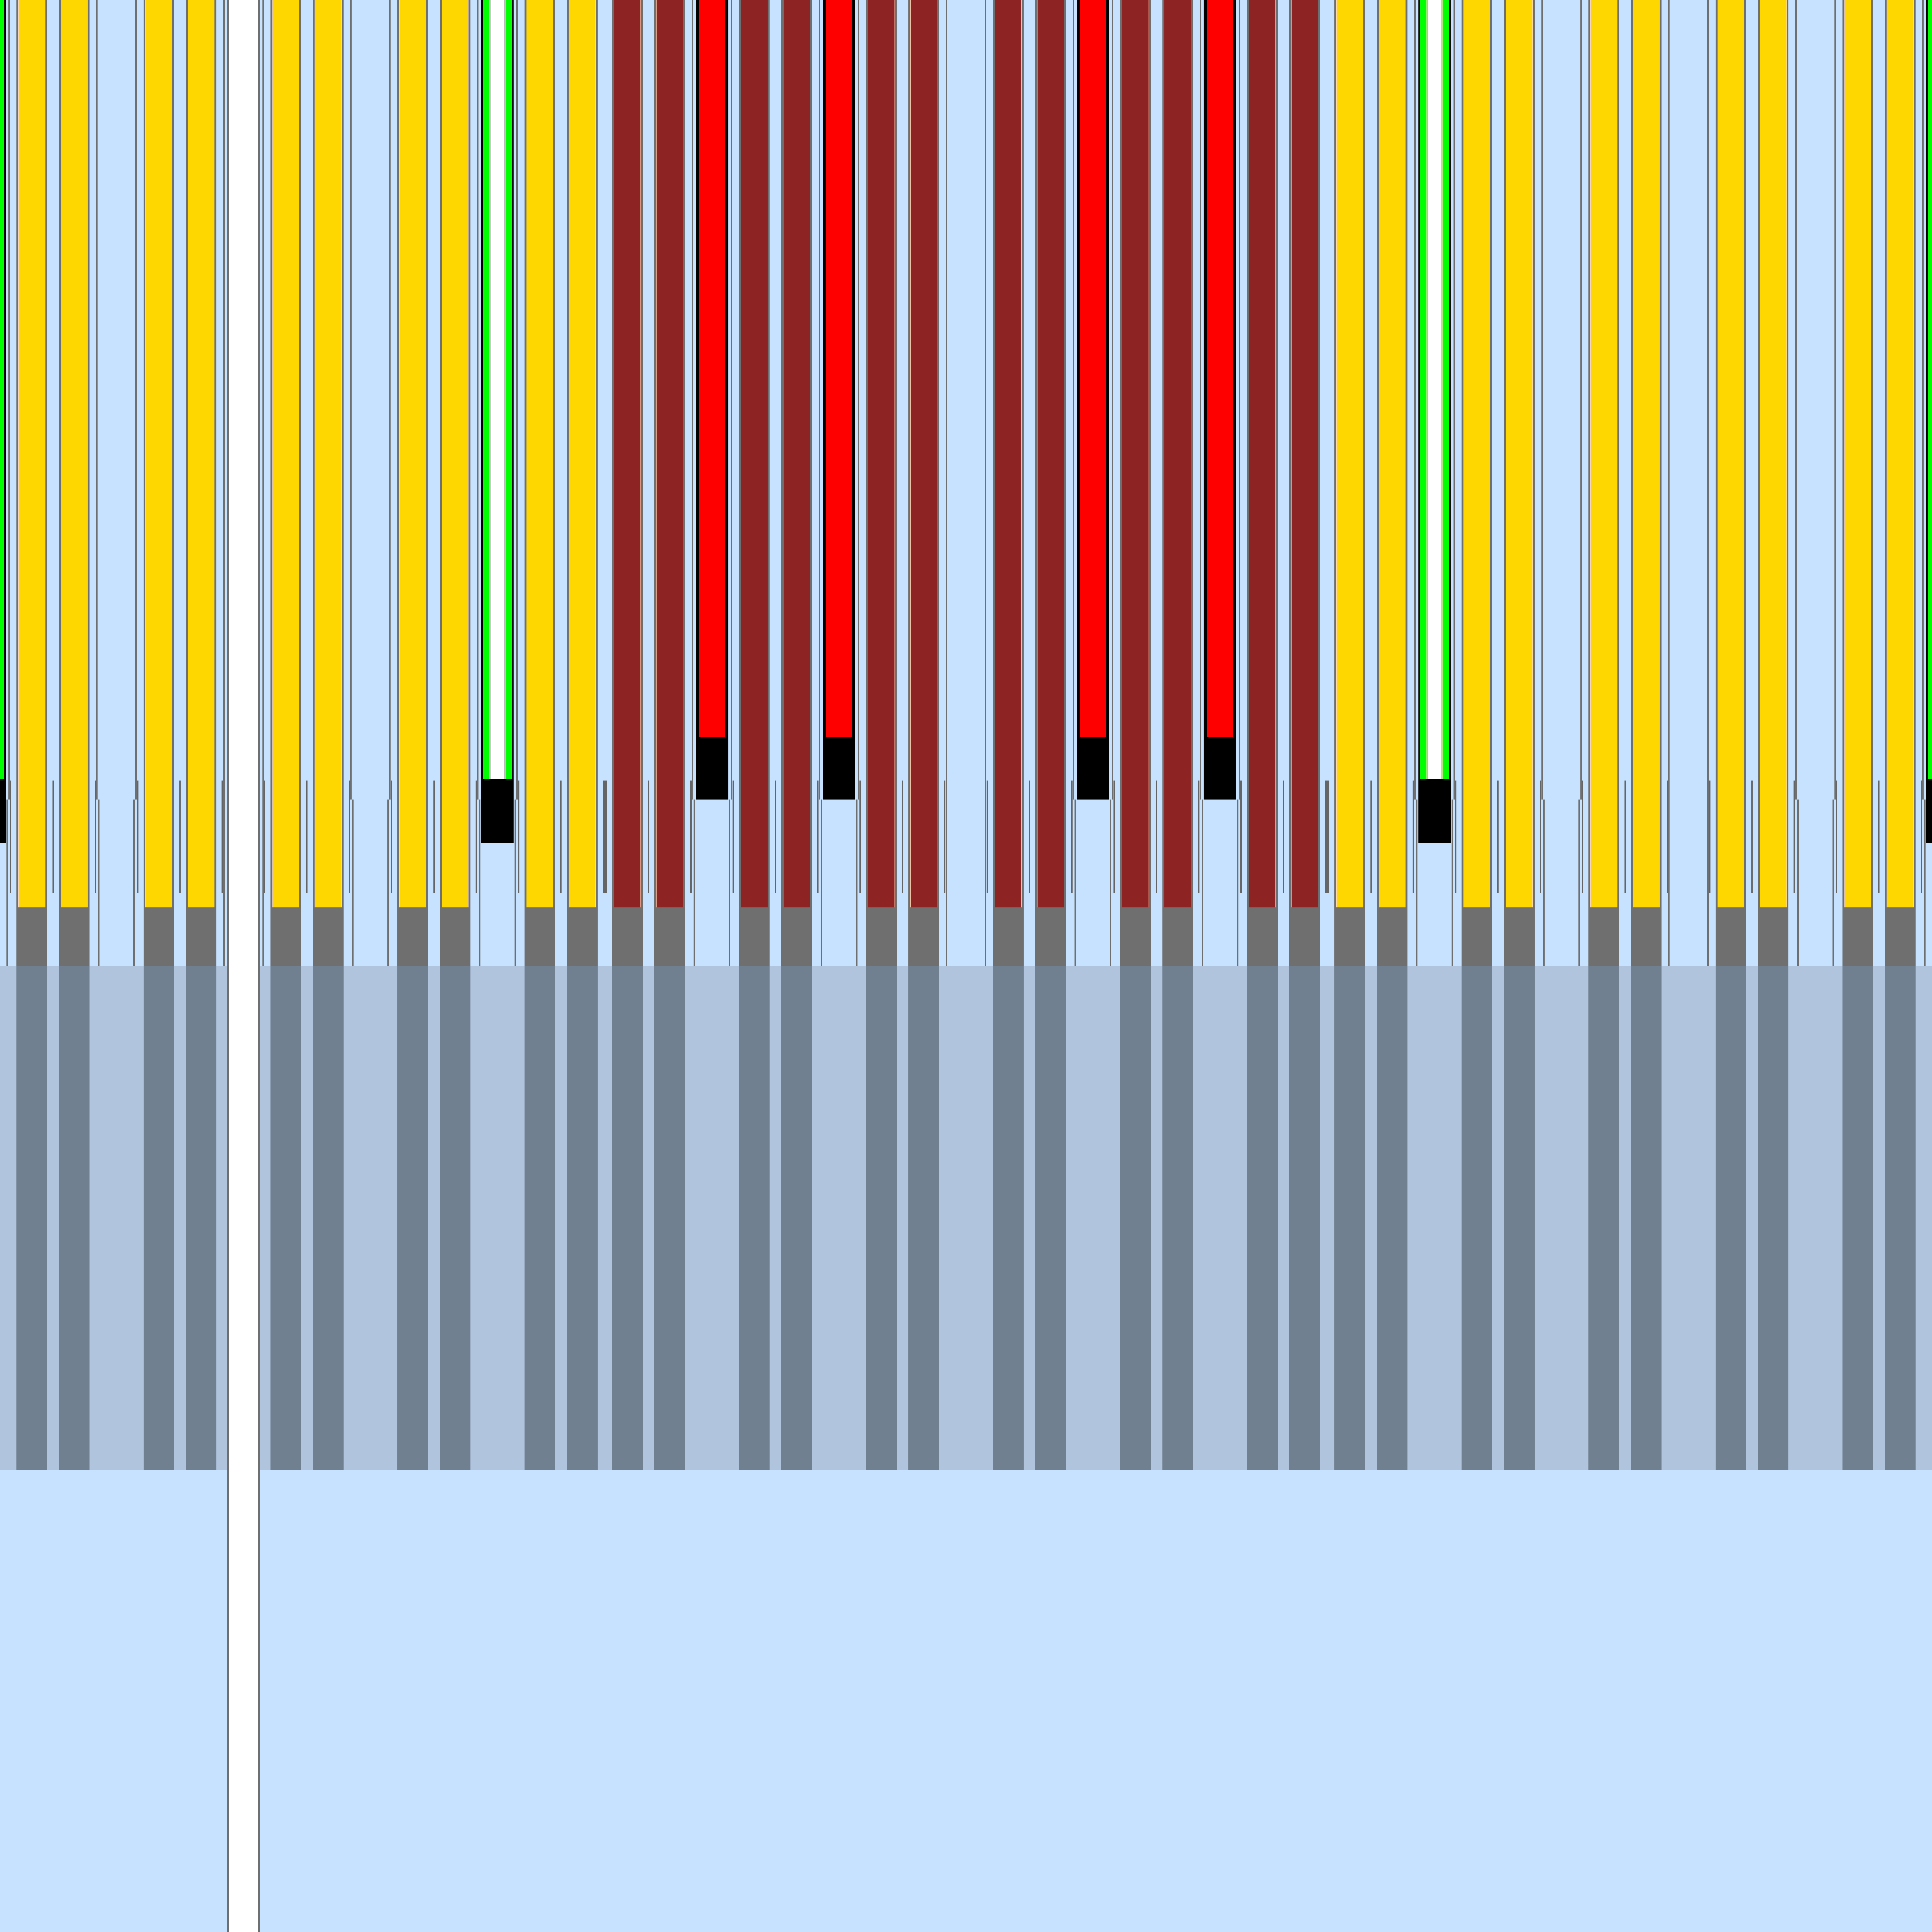
\includegraphics[height=\height cm]{specifications/axial/figs/axial_mats_row_8_botzoom.png}};

      % real geometries of the plots
      \def\realtopcenter{419.704}
      \def\realbotcenter{35.00}
      \def\realheight{57.5}
      
      \def\f{\height/\realheight}

      \def\n{20} % number of planes

      \foreach \a/\l/\c/\rc/\i in {20.0000/Bottom of Support Plate/botpic/\realbotcenter/1,
                            35.0000/Bottom of Fuel Rod/botpic/\realbotcenter/2,
                            36.7480/Bottom of Active Fuel/botpic/\realbotcenter/3,
                            37.1621/Grid 1 Bottom/botpic/\realbotcenter/4,
                            38.6600/Bottom of BPRA Rod/botpic/\realbotcenter/5,
                            39.9580/Bottom of Fully-Inserted RCCA Rod/botpic/\realbotcenter/6,
                            40.5200/Grid 1 Top/botpic/\realbotcenter/7,
                            40.5580/Bottom of BPRA Rod Absorber/botpic/\realbotcenter/8,
                            41.8280/Bottom of RCCA Rod Lower Absorber/botpic/\realbotcenter/9,
                            401.238/Top of BPRA Rod Absorber/toppic/\realtopcenter/10,
                            402.508/Top of Active Fuel/toppic/\realtopcenter/11,
                            403.778/Bottom of RCCA Rod Upper Plenum/toppic/\realtopcenter/12,
                            411.806/Grid 8 Bottom/toppic/\realtopcenter/13,
                            415.164/Grid 8 Top/toppic/\realtopcenter/14,
                            415.558/Top of RCCA Rod Upper Plenum/toppic/\realtopcenter/15,
                            417.164/Top of Fuel Rod Upper Plenum/toppic/\realtopcenter/16,
                            419.704/Top of Fuel Rod/toppic/\realtopcenter/17,
                            421.532/Top of BPRA Rod Upper Plenum/toppic/\realtopcenter/18,
                            423.049/Bottom of Upper Nozzle/toppic/\realtopcenter/19,
                            431.876/Top of Upper Nozzle/toppic/\realtopcenter/20
                            }
          \draw[red,thick] let \p{A}=(\c.west) in 
              (\x{A},\y{A}+\f*\a cm - \f*\rc cm) -- 
                  ++(\height+0.5,0) -- (\height/2+1.25,\i-\height*1.7) -- ++(0.75,0)
                      node[black,right,anchor=west,font=\scriptsize] {\l};

    \end{tikzpicture}
    
    \caption[Axial scale view of aggregate pincell model near core top and
    bottom]{Axial scale view of the model near the top and bottom of the fuel
    rods in row 8, showing pin plenums, approximated
    springs, end plugs, and structures. \emph{Blue}: water; \emph{orange}: helium;
    \emph{black}: stainless steel; \emph{dark gray}: Zircaloy; \emph{dim gray}
    Inconel; \emph{white}: air; \emph{slate gray}: nozzle / support plate
    stainless steel; \emph{steel blue}: nozzle / support plate borated water;
    \emph{green}: borosilicate glass; \emph{yellow}: fuel. \label{fig:tb_detail}}
\end{figure}

